\documentclass[11pt,a4paper,twoside,openany]{book}
\usepackage[a4paper,left=28mm,right=28mm,top=27mm,bottom=26mm,headsep=8mm]{geometry}
% Shared look of the Rakshasutra white paper and book.
\usepackage[T1]{fontenc}
\usepackage[utf8]{inputenc}
\usepackage{charter}
\usepackage[scaled=0.9]{helvet}
\usepackage{courier}
\usepackage{amsmath,amssymb}
\usepackage{graphicx}
\usepackage{booktabs,array,longtable}
\usepackage[table]{xcolor}
\usepackage{textcomp}
\usepackage{enumitem}
\usepackage{microtype}
\usepackage{tikz}
\usetikzlibrary{arrows.meta,positioning}
\usepackage[most]{tcolorbox}
\definecolor{rsink}{HTML}{171A2B}
\definecolor{rsred}{HTML}{C0271D}
\definecolor{rspaper}{HTML}{F6F1E7}
\definecolor{rsmuted}{HTML}{6A6F85}
\definecolor{rsindigo}{HTML}{2F4B9A}
\definecolor{rsrule}{HTML}{D9D2C2}
\usepackage[colorlinks=true,allcolors=rsindigo]{hyperref}
\usepackage{xurl}
\urlstyle{same}
% Written by generated/make_numbers.py from results/summary.json. Do not edit.
\newcommand{\ToaSos}{66.82}
\newcommand{\ToaBloom}{138.50}
\newcommand{\ToaChunk}{338.18}
\newcommand{\ToaSosNine}{226.3}
\newcommand{\LossSingle}{57.6}
\newcommand{\LossBatch}{25.3}
\newcommand{\LossRak}{30.5}
\newcommand{\LossRakNd}{21.3}
\newcommand{\LoadSingle}{42.9}
\newcommand{\LoadBatch}{14.6}
\newcommand{\LoadRak}{18.2}
\newcommand{\LoadRakNd}{12.0}
\newcommand{\LossRakLow}{14.3}
\newcommand{\LossRakNdLow}{9.7}
\newcommand{\LossBatchLow}{8.6}
\newcommand{\OversizeBatch}{22}
\newcommand{\LossChunk}{34}
\newcommand{\AirRed}{57.6}
\newcommand{\AirRedNd}{72.1}
\newcommand{\AirVsBatch}{25}
\newcommand{\AirVsBatchNd}{18}
\newcommand{\BloomPays}{960}
\newcommand{\DepTags}{637}
\newcommand{\DepPoles}{32}
\newcommand{\DepLoss}{11.0}
\newcommand{\DepLossNd}{7.3}
\newcommand{\McFrames}{695{,}304}
\newcommand{\McErr}{1.7}
\newcommand{\RangeAbove}{4.1}
\newcommand{\RangeOneM}{82}
\newcommand{\RangeCoded}{174}
\newcommand{\MarginFifty}{20.3}
\newcommand{\Mapl}{145.4}
\newcommand{\MaplUnder}{124.9}
\newcommand{\MarginEightOver}{16.1}
\newcommand{\MarginEightUnder}{4.4}
\newcommand{\MarginFourUnder}{1.7}
\newcommand{\MarginFourOver}{22.2}
\newcommand{\GateTrackM}{22}
\newcommand{\GateHubM}{7.5}
\newcommand{\Iactive}{29.74}
\newcommand{\LifeWarm}{48.2}
\newcommand{\LifeCold}{33.8}
\newcommand{\AdvCoded}{5.95}
\newcommand{\AdvOneM}{0.79}
\newcommand{\IactiveCoded}{113.2}
\newcommand{\LifeWarmCoded}{12.8}
\newcommand{\LifeColdCoded}{9.0}
\newcommand{\DroopUnbuf}{1.61}
\newcommand{\DroopCap}{1.61}
\newcommand{\CapNeed}{895}
\newcommand{\PulseMax}{29.8}
\newcommand{\TauMs}{4.2}
\newcommand{\TetherHit}{0.48}
\newcommand{\TetherAlarm}{98}
\newcommand{\TetherAlarmSim}{98}
\newcommand{\TetherWindow}{811}
\newcommand{\TetherUa}{746}
\newcommand{\ParentLife}{1.9}
\newcommand{\TetherRange}{174}
\newcommand{\TetherGate}{78}
\newcommand{\EvCap}{99.7}
\newcommand{\EvCapDense}{95.0}
\newcommand{\SlowTwo}{25}
\newcommand{\SlowFiveOne}{90}
\newcommand{\ClassAWalk}{216}
\newcommand{\SosMedian}{0.5}
\newcommand{\SosFour}{92}
\newcommand{\SosFirstLoss}{23}
\newcommand{\SosPninefive}{7.0}
\newcommand{\SosFiberP}{0.6}
\newcommand{\SosFourLow}{96}
\newcommand{\BloomFifty}{1.6}
\newcommand{\BloomHundred}{8.7}
\newcommand{\BloomThree}{57}
\newcommand{\BloomCapFive}{78}
\newcommand{\BloomCapOne}{41}
\newcommand{\Clash}{10}
\newcommand{\WalkSepDelay}{105}
\newcommand{\WalkSepM}{243}
\newcommand{\WalkSosDelay}{0.3}
\newcommand{\WalkUplinks}{151}
\newcommand{\BranchExample}{3.0}
\newcommand{\AuditRep}{16}
\newcommand{\AuditDiff}{16}
\newcommand{\AuditFix}{6}
\newcommand{\AuditOpen}{4}
\newcommand{\AuditTotal}{42}
\newcommand{\Ntests}{104}
\newcommand{\Nparams}{97}
\newcommand{\Nassumed}{10}
\newcommand{\Ndefined}{5}
\newcommand{\Npaper}{78}
\newcommand{\Nstandard}{4}
\newcommand{\LossSingleLow}{14.1}
\newcommand{\LoadRakNdFrac}{0.120}
\newcommand{\LossRakNdFrac}{0.213}

% Written by generated/make_numbers.py. Do not edit.
\newcommand{\TableCapacity}{\begin{tabular}{@{}p{0.25\linewidth}rrrrl@{}}\toprule
Forwarding design & 500 & 1,000 & 2,000 & 3,000 & Largest frame\\\midrule
Raw forwarding (2 s pings) & 176.8 / 97.1 & 353.6 / 99.9 & 707.2 / 100.0 & 1060.8 / 100.0 & 7 B \\
Single-event arrivals + raw ID heartbeat & 7.6 / 14.1 & 14.6 / 25.4 & 28.7 / 43.7 & 42.9 / 57.6 & over 222 B \\
15 s batching + raw ID heartbeat & 4.5 / 8.6 & 6.7 / 12.5 & 10.6 / 19.0 & 14.6 / 25.3 & over 222 B \\
Rakshasutra as specified & 7.7 / 14.3 & 10.2 / 18.4 & 14.2 / 24.7 & 18.2 / 30.5 & $\leq$ 200 B \\
Rakshasutra without departure lists & 5.1 / 9.7 & 6.6 / 12.4 & 9.3 / 17.0 & 12.0 / 21.3 & $\leq$ 200 B \\
\bottomrule\end{tabular}}
\newcommand{\TableCapacityCompare}{\begin{tabular}{@{}p{0.36\linewidth}ll@{}}\toprule
Forwarding design & First draft, loss (\%) & This model, loss (\%)\\\midrule
Raw forwarding (2 s pings) & 97.7 / 99.9 / 100 / 100 & 97.1 / 99.9 / 100.0 / 100.0 \\
Single-event arrivals + raw ID heartbeat & 12.2 / 22.9 / 40.5 / 54.2 & 14.1 / 25.4 / 43.7 / 57.6 \\
15 s batching + raw ID heartbeat & 5.8 / 11.3 / 16.8 / 22.1 & 8.6 / 12.5 / 19.0 / 25.3 \\
Rakshasutra as specified & 4.1 / 8.1 / 12.0 / 15.8 & 14.3 / 18.4 / 24.7 / 30.5 \\
Rakshasutra without departure lists & -- & 9.7 / 12.4 / 17.0 / 21.3 \\
\bottomrule\end{tabular}}
\newcommand{\TableLink}{\begin{tabular}{@{}p{0.30\linewidth}lrrrl@{}}\toprule
Link & PHY & $P_{tx}$ & Roof & $S_{rx}$ & Range or margin\\\midrule
Wearable to pole, pole above the roof & BLE 1M & +4 & 24.1 & -96.0 & 4.1 m \\
Wearable to pole, pole under the roof & BLE 1M & +8 & 0.0 & -96.0 & 82.2 m \\
Wearable to pole, pole under the roof & BLE Coded S=8 & +8 & 0.0 & -103.0 & 174.1 m \\
Pole to gateway, antenna under the roof & LoRa SF7 & +14 & 18.4 & -126.5 & -4.4 dB \\
Pole to gateway, whip above the roof & LoRa SF7 & +14 & 0.0 & -126.5 & +16.1 dB \\
\bottomrule\end{tabular}}
\newcommand{\TablePower}{\begin{tabular}{@{}p{0.27\linewidth}lrrr@{}}\toprule
State & Interval & Peak, mA & On, ms & Mean, \textmu A\\\midrule
Sleep, 32.768 kHz clock and RAM retention & continuous & 0.0018 & -- & 1.80 \\
Signed advertisement & every 0.8 s & 14.2 & 1.25 & 22.19 \\
Scan window for a wake token & every 4 s & 4.6 & 5 & 5.75 \\
AES-CMAC slot rotation & every 900 s & 3.8 & 0.45 & 0.00 \\
\midrule Total on the trek &&&& 29.74 \\
\bottomrule\end{tabular}}
\newcommand{\TableZones}{\begin{tabular}{@{}llrrrl@{}}\toprule
Zone & Segments & km & Poles & Spacing (m) & Backhaul\\\midrule
1 & old-track & 6.0 & 56 & 107 & LoRaWAN \\
2 & tarakote & 7.0 & 65 & 108 & LoRaWAN \\
3 & adhkuwari & 0.5 & 20 & 25 & fibre LAN \\
4 & himkoti + sanjichhat & 6.5 & 60 & 108 & LoRaWAN \\
5 & bhawan & 1.0 & 40 & 25 & fibre LAN \\
6 & bhairon & 1.5 & 14 & 107 & LoRaWAN \\
\midrule & Total & 22.5 & 255 & & \\\bottomrule\end{tabular}}
\newcommand{\TableAudit}{\begin{longtable}{@{}lp{0.40\linewidth}p{0.13\linewidth}p{0.21\linewidth}l@{}}\toprule
& Claim & First draft & This model & Verdict\\\midrule\endhead
A01 & Time on air, SOS frame (15 B, SF7) & 66.82 & 66.82 ms & reproduced \\
A02 & Time on air, Bloom heartbeat (64 B, SF7) & 138.5 & 138.5 ms & reproduced \\
A03 & Time on air, 25-tag chunk (200 B, SF7) & 338.18 & 338.18 ms & reproduced \\
A04 & Pseudonyms that fit one raw 222-byte list & 55 & 55 IDs & reproduced \\
A05 & Maximum allowable LoRa path loss, whip above the roof & 145.4 & 145.4 dB & reproduced \\
A06 & BLE Coded PHY margin at 50 m, heavy crowd & 28.6 & 20.3 dB & differs \\
A07 & BLE range at 98\% delivery, pole above the roof, 1M PHY, +4 dBm & 4.2 & 4.1 m & reproduced \\
A08 & BLE range at 98\% delivery, pole under the roof, 1M PHY & 28.5 & 82.2 m & differs \\
A09 & BLE range at 98\% delivery, pole under the roof, Coded PHY & 92.0 & 174.0 m & differs \\
A10 & LoRa range, whip above the roof & 5.4-8.8 km & 16.1 dB margin at 8 km  & open \\
A11 & LoRa range, antenna under the roof & 0.85 km & -4.4 dB margin at 8 km  & open \\
A12 & Uplink loss, raw forwarding, 500 tags in the cell & 97.7 & 97.1 \% & reproduced \\
A13 & Uplink loss, raw forwarding, 3,000 tags in the cell & 100.0 & 100.0 \% & reproduced \\
A14 & Uplink loss, single-event arrivals, 500 tags in the cell & 12.2 & 14.1 \% & differs \\
A15 & Uplink loss, single-event arrivals, 3,000 tags in the cell & 54.2 & 57.6 \% & differs \\
A16 & Uplink loss, 15 s batching, 500 tags in the cell & 5.8 & 8.6 \% & differs \\
A17 & Uplink loss, 15 s batching, 3,000 tags in the cell & 22.1 & 25.3 \% & differs \\
A18 & Uplink loss, Rakshasutra, 500 tags in the cell & 4.1 & 14.3 \% & differs \\
A19 & Uplink loss, Rakshasutra, 3,000 tags in the cell & 15.8 & 30.5 \% & differs \\
A20 & Uplink loss, Rakshasutra without departure lists, 3,000 tags & 15.8 & 21.3 \% & design fix \\
A21 & Reduction in LoRa airtime, 3,000 tags & 82.4 & 57.6 \% & differs \\
A22 & Uplink loss in the deployed layout, 5,000 tags on the trek & $<$ 6 & 11.0 \% & differs \\
A23 & Class A worst-case alert delay & 173 & 173.0 s & reproduced \\
A24 & Distance walked during that delay & 215 & 216 m & reproduced \\
A25 & Time an EV passenger spends in a 25 m core zone & 4.5 & 4.5 s & reproduced \\
A26 & EV capture with one decoded frame required & 99.4 & 99.7 \% & reproduced \\
A27 & Tether: chance one 5 ms scan hears the child's band & assumed 1 & 0.48 \% & design fix \\
A28 & Tether: separation at which the alert sounds & 25-30 m & 174 m  & design fix \\
A29 & Mean current on the trek (Table V) & 29.74 & 29.74 uA & reproduced \\
A30 & Battery life at 25\,\textdegree C, from Table V & 14.2 & 48.2 months & differs \\
A31 & Battery life at $-5$\,\textdegree C, from Table V & 11.1 & 33.8 months & differs \\
A32 & Transmit time per advertisement on Coded PHY & 1.25 & 5.95 ms & differs \\
A33 & Supply during an unbuffered buzzer pulse at $-5$\,\textdegree C & 1.61 & 1.61 V & reproduced \\
A34 & Supply during the pulse with the 100 \textmu F capacitor & 2.68 & 1.61 V & design fix \\
A35 & Chance of forging an SOS in one try & 2.33e-10 & 2.33e-10  & reproduced \\
A36 & Chance of forging a wake token in one try & 5.96e-08 & 5.96e-08  & reproduced \\
A37 & Pseudonyms are unique in the lookup table & assumed & 10\% chance of a clash  & design fix \\
A38 & Replayed frames are rejected & all & outside the 3-slot window  & design fix \\
A39 & Bloom heartbeat false-positive rate & not stated & 1.6\% at 50 tags, 57\% at 300  & open \\
A40 & Pole spacing on the LoRa tracks & 25-100 m & 108 m  & differs \\
A41 & Wearable transmit power on the nRF52811 & +8 dBm & +4 dBm  & open \\
A42 & SOS reaches the control room within 4 s (3,000-tag surge) & all & 92\% (median 0.5 s)  & differs \\
\bottomrule\end{longtable}}
\newcommand{\TableParams}{\begin{longtable}{@{}p{0.25\linewidth}p{0.14\linewidth}lp{0.31\linewidth}@{}}\toprule
Parameter & Value & Status & Source or note\\\midrule\endhead
\texttt{trek\_km} & \raggedright 22.5 km & paper & WP-01 Sec. III-A, total of the six zones \\
\texttt{poles\_total} & \raggedright 255 poles & paper & WP-01 Sec. III-A \\
\texttt{poles\_fiber} & \raggedright 60 poles & paper & WP-01 Sec. V-D; zones 3 and 5 on the fibre LAN \\
\texttt{gateways} & \raggedright 6 gateways & paper & WP-01 Sec. III-B \\
\texttt{altitude\_min\_m} & \raggedright 762.0 m & paper & WP-01 Sec. III-A (2,500 ft) \\
\texttt{altitude\_max\_m} & \raggedright 2017.0 m & paper & WP-01 Sec. III-A (6,619 ft) \\
\texttt{zone4\_himkoti\_km} & \raggedright 3.5 km & assumed & split of the 6.5 km of zone 4 between its two parallel branches \\
\texttt{zone4\_sanjichhat\_km} & \raggedright 3.0 km & assumed & split of the 6.5 km of zone 4 between its two parallel branches \\
\texttt{ble\_tx\_dbm} & \raggedright 8.0 dBm & paper & WP-01 Eq. 2; note the nRF52811 named in the paper is specified to +4 dBm \\
\texttt{ble\_tx\_dbm\_1m\_above} & \raggedright 4.0 dBm & paper & WP-01 Table III, first row \\
\texttt{ble\_pl0\_db} & \raggedright 40.2 dB & paper & WP-01 Eq. 2, path loss at 1 m \\
\texttt{ble\_exponent} & \raggedright 2.15  & paper & WP-01 Eq. 2, under the steel roof; not measured \\
\texttt{ble\_sigma\_db} & \raggedright 4.2 dB & paper & WP-01 Eq. 2, log-normal shadowing \\
\texttt{ble\_body\_db} & \raggedright 14.0 dB & paper & WP-01 Table III, heavy crowd \\
\texttt{ble\_antenna\_gain\_db} & \raggedright 0.0 dB & assumed & sum of wearable and pole antenna gains; the paper gives none \\
\texttt{ble\_sens\_1m\_dbm} & \raggedright -96.0 dBm & paper & WP-01 Table III \\
\texttt{ble\_sens\_coded\_dbm} & \raggedright -103.0 dBm & paper & WP-01 Eq. 2, Coded PHY S=8 on ESP32-S3 \\
\texttt{gi\_loss\_ble\_db} & \raggedright 24.1 dB & paper & WP-01 Sec. III-B, roof penetration at 2.44 GHz; not measured \\
\texttt{gi\_loss\_lora\_db} & \raggedright 18.4 dB & paper & WP-01 Sec. III-B, roof penetration at 866 MHz; not measured \\
\texttt{pdr\_target} & \raggedright 0.98  & paper & WP-01 Table III, 'reliable range' means at least 98\% delivery \\
\texttt{lora\_tx\_dbm} & \raggedright 14.0 dBm & paper & WP-01 Sec. III-B \\
\texttt{lora\_coax\_db} & \raggedright 0.9 dB & paper & WP-01 Sec. III-B, 1 m of RG-316 \\
\texttt{lora\_gw\_gain\_dbi} & \raggedright 5.8 dBi & paper & WP-01 Sec. III-B \\
\texttt{lora\_sens\_sf7\_dbm} & \raggedright -126.5 dBm & paper & WP-01 Sec. III-B, SX1302 \\
\texttt{lora\_sens\_sf9\_dbm} & \raggedright -131.5 dBm & paper & WP-01 Sec. III-B, SX1302 \\
\texttt{lora\_freq\_mhz} & \raggedright 866.0 MHz & standard & centre of IN865, LoRa Alliance RP002-1.0.4 \\
\texttt{lora\_body\_internal\_db} & \raggedright 3.0 dB & paper & WP-01 Table III, internal antenna under the roof \\
\texttt{ridge\_loss\_db} & \raggedright 20.0 dB & assumed & one knife-edge ridge between pole and gateway \\
\texttt{lora\_channels} & \raggedright 8 channels & paper & WP-01 Sec. V-A \\
\texttt{lora\_mac\_overhead} & \raggedright 13 bytes & standard & LoRaWAN MHDR, FHDR, FPort and MIC \\
\texttt{lora\_max\_app\_bytes} & \raggedright 222 bytes & standard & IN865 DR5, repeater-compatible; RP002-1.0.4 \\
\texttt{cell\_poles} & \raggedright 60 poles & paper & WP-01 Sec. VI-B \\
\texttt{pass\_seconds} & \raggedright 55.0 s & paper & WP-01 Sec. VI-B, mean time between poles \\
\texttt{raw\_ping\_seconds} & \raggedright 2.0 s & paper & WP-01 Table IV, row 1 \\
\texttt{raw\_ping\_bytes} & \raggedright 7 bytes & assumed & 6-byte MAC and 1-byte RSSI per forwarded ping \\
\texttt{arrival\_tuple\_bytes} & \raggedright 8 bytes & paper & WP-01 Algorithm 2, line 12 \\
\texttt{departure\_bytes} & \raggedright 4 bytes & paper & WP-01 Algorithm 2, line 17 \\
\texttt{chunk\_tags} & \raggedright 25 tags & paper & WP-01 Algorithm 2, line 16 \\
\texttt{departure\_ids\_per\_frame} & \raggedright 50 ids & paper & WP-01 Algorithm 2, line 17 \\
\texttt{flush\_seconds} & \raggedright 15.0 s & paper & WP-01 Algorithm 2 \\
\texttt{heartbeat\_seconds} & \raggedright 60.0 s & paper & WP-01 Algorithm 2 \\
\texttt{depart\_timeout\_s} & \raggedright 90.0 s & paper & WP-01 Algorithm 2, line 15 \\
\texttt{rssi\_gate\_track\_dbm} & \raggedright -75.0 dBm & paper & WP-01 Algorithm 2, line 8 \\
\texttt{rssi\_gate\_hub\_dbm} & \raggedright -65.0 dBm & paper & WP-01 Algorithm 2, line 8 \\
\texttt{sos\_per\_minute} & \raggedright 10 frames & paper & WP-01 Algorithm 2, line 3 \\
\texttt{adv\_interval\_s} & \raggedright 0.8 s & paper & WP-01 Sec. IV-C \\
\texttt{adv\_interval\_sos\_s} & \raggedright 0.2 s & paper & WP-01 Sec. IV-C \\
\texttt{slot\_seconds} & \raggedright 900 s & paper & WP-01 Sec. IV-C \\
\texttt{walk\_mps} & \raggedright 1.25 m/s & paper & WP-01 Sec. V-C \\
\texttt{ev\_mps} & \raggedright 5.56 m/s & paper & WP-01 Sec. V-C (20 km/h) \\
\texttt{core\_zone\_m} & \raggedright 25.0 m & paper & WP-01 Sec. V-C, length of track a pole reports as 'here' \\
\texttt{class\_a\_batch\_s} & \raggedright 15.0 s & paper & WP-01 Sec. V-C \\
\texttt{class\_a\_confirm\_s} & \raggedright 90.0 s & paper & WP-01 Sec. V-C \\
\texttt{class\_a\_downlink\_s} & \raggedright 60.0 s & paper & WP-01 Sec. V-C \\
\texttt{class\_a\_gatt\_s} & \raggedright 8.0 s & paper & WP-01 Sec. V-C \\
\texttt{tether\_scan\_period\_s} & \raggedright 5.0 s & paper & WP-01 Sec. V-C, Layer 1 \\
\texttt{tether\_scan\_window\_s} & \raggedright 0.005 s & paper & WP-01 Sec. V-C, Layer 1 \\
\texttt{tether\_misses} & \raggedright 4 scans & paper & WP-01 Sec. V-C, Layer 1 \\
\texttt{adv\_delay\_max\_s} & \raggedright 0.01 s & standard & Bluetooth Core 5.1, random advDelay of 0 to 10 ms \\
\texttt{separation\_alert\_m} & \raggedright 200.0 m & paper & WP-01 Sec. V-C, Layer 2 \\
\texttt{suspect\_speed\_mps} & \raggedright 8.0 m/s & assumed & above the 5.56 m/s of an electric vehicle; faster sightings are flagged \\
\texttt{suspect\_min\_m} & \raggedright 300.0 m & assumed & shorter hops are within radio range of two poles and are not flagged \\
\texttt{class\_c\_downlink\_s} & \raggedright 1.0 s & assumed & server decision, network server and one Class C downlink \\
\texttt{lorawan\_retry\_s} & \raggedright 3.0 s & assumed & wait before a confirmed uplink is repeated (RX2 window plus back-off) \\
\texttt{backhaul\_s} & \raggedright 0.3 s & assumed & gateway to control-room alarm \\
\texttt{battery\_mah} & \raggedright 620.0 mAh & paper & WP-01 Table V, CR2450 \\
\texttt{battery\_cold\_derate} & \raggedright 0.3  & paper & WP-01 Sec. VI-C, capacity lost at $-5$\,\textdegree C \\
\texttt{battery\_r\_warm\_ohm} & \raggedright 15.0 ohm & paper & WP-01 Sec. VI-C \\
\texttt{battery\_r\_cold\_ohm} & \raggedright 42.0 ohm & paper & WP-01 Sec. VI-C \\
\texttt{battery\_v\_cold} & \raggedright 2.95 V & paper & WP-01 Sec. VI-C, open-circuit voltage at $-5$\,\textdegree C \\
\texttt{brownout\_v} & \raggedright 1.7 V & paper & WP-01 Sec. VI-C, nRF52811 minimum supply \\
\texttt{i\_sleep\_ua} & \raggedright 1.8 uA & paper & WP-01 Table V \\
\texttt{i\_tx\_ma} & \raggedright 14.2 mA & paper & WP-01 Table V \\
\texttt{t\_tx\_ms} & \raggedright 1.25 ms & paper & WP-01 Table V; matches a 1M PHY event on three channels, not Coded PHY \\
\texttt{i\_rx\_ma} & \raggedright 4.6 mA & paper & WP-01 Table V \\
\texttt{t\_scan\_ms} & \raggedright 5.0 ms & paper & WP-01 Table V \\
\texttt{scan\_period\_ms} & \raggedright 4000.0 ms & paper & WP-01 Table V \\
\texttt{i\_cmac\_ma} & \raggedright 3.8 mA & paper & WP-01 Table V \\
\texttt{t\_cmac\_ms} & \raggedright 0.45 ms & paper & WP-01 Table V \\
\texttt{i\_rack\_ua} & \raggedright 0.6 uA & paper & WP-01 Table V \\
\texttt{active\_hours} & \raggedright 14.0 h/day & paper & WP-01 Sec. VI-C \\
\texttt{i\_pulse\_ma} & \raggedright 32.0 mA & paper & WP-01 Sec. VI-C, buzzer and LED \\
\texttt{holdup\_uf} & \raggedright 100.0 uF & paper & WP-01 Sec. VI-C \\
\texttt{pulse\_on\_ms} & \raggedright 100.0 ms & paper & WP-01 Sec. VI-C \\
\texttt{pulse\_off\_ms} & \raggedright 400.0 ms & paper & WP-01 Sec. VI-C \\
\texttt{company\_id} & \raggedright 65370  & paper & WP-01 Table II, laboratory identifier \\
\texttt{bloom\_bits} & \raggedright 512 bits & paper & WP-01 Algorithm 2 \\
\texttt{bloom\_probes} & \raggedright 3  & paper & WP-01 Algorithm 2, lines 20-22 \\
\texttt{active\_table} & \raggedright 1024 entries & paper & WP-01 Algorithm 2 \\
\texttt{window\_slots} & \raggedright 3 slots & paper & WP-01 Sec. IV-D \\
\texttt{arbitration\_s} & \raggedright 15.0 s & paper & WP-01 Algorithm 1, line 12 \\
\texttt{crystal\_ppm} & \raggedright 20.0 ppm & paper & WP-01 Sec. IV-D \\
\texttt{truncation} & \raggedright leading bytes  & defined & Trunc keeps the first bytes of the CMAC, as in RFC 4493 \\
\texttt{counter\_encoding} & \raggedright little-endian  & defined & the counter enters every CMAC input as it appears on air \\
\texttt{wake\_token\_layout} & \raggedright id4\textbar{}cmd1\textbar{}tag3  & defined & the paper fixes 8 bytes and 24 bits of tag only \\
\texttt{sos\_uplink\_layout} & \raggedright frame15\textbar{}rssi1  & defined & one RSSI byte is appended so the server can pick the nearest pole \\
\texttt{bloom\_hashes} & \raggedright CRC-16/CCITT-FALSE, FNV-1a 32  & defined & the paper names CRC16 and FNV1a without variants \\
\bottomrule\end{longtable}}

\graphicspath{{../generated/fig/}}
\setlist{nosep,leftmargin=1.4em,topsep=3pt}
\renewcommand{\arraystretch}{1.18}
\arrayrulecolor{rsink}
\newcommand{\code}[1]{\texttt{#1}}
\newcommand{\Kmaster}{K_{\mathrm{master}}}
\newcommand{\cmac}[2]{\operatorname{CMAC}_{#1}\!\left(#2\right)}
\newcommand{\simnote}{\textsf{\footnotesize\color{rsmuted}calculated}}
% A box for a finding or a caveat
\newtcolorbox{finding}[1][]{enhanced,breakable,colback=rspaper,colframe=rspaper,boxrule=0pt,arc=0pt,left=9pt,right=9pt,
  top=6pt,bottom=6pt,borderline west={2.4pt}{0pt}{rsred},fontupper=\small,#1}
\newtcolorbox{algo}[1]{enhanced,breakable,colback=white,colframe=rsink,boxrule=0.5pt,arc=0pt,left=6pt,right=6pt,top=5pt,
  bottom=5pt,title={\sffamily\small\bfseries #1},coltitle=white,colbacktitle=rsink,fontupper=\footnotesize}
% the thread: a twisted two-strand rule
\newcommand{\thread}[1][\linewidth]{\par\noindent\begin{tikzpicture}\draw[rsred,line width=1.1pt,line cap=butt](0,0)--(\dimexpr#1-1.2pt\relax,0);
  \foreach \x in {0.5}{\fill[rsred](\x*#1,0) circle(2.1pt);\fill[white](\x*#1,0) circle(0.9pt);}\end{tikzpicture}\par}

\usepackage{titlesec}
\usepackage{fancyhdr}
\usepackage{caption}
\usepackage{placeins}
\captionsetup{font={small,sf},labelfont={bf,color=rsred},labelsep=quad,justification=raggedright,singlelinecheck=false}
\captionsetup[table]{position=top}
\titleformat{\chapter}[display]{\normalfont\sffamily\color{rsink}}
  {\fontsize{9}{11}\selectfont\bfseries\color{rsmuted}\MakeUppercase{\chaptertitlename}\ \thechapter}{4pt}
  {\raggedright\fontsize{26}{30}\selectfont\bfseries}[\vspace{6pt}\thread]
\titlespacing*{\chapter}{0pt}{0pt}{18pt}
\titleformat{\section}{\sffamily\bfseries\large\color{rsink}}{\color{rsred}\thesection}{0.7em}{}
\titleformat{\subsection}{\sffamily\bfseries\normalsize\color{rsink}}{\thesubsection}{0.7em}{}
\pagestyle{fancy}\fancyhf{}
\fancyhead[LE]{\sffamily\small\bfseries\thepage\hfill\mdseries\color{rsmuted}A Thread Through the Crowd}
\fancyhead[RO]{\sffamily\small\color{rsmuted}\nouppercase{\leftmark}\hfill\color{black}\bfseries\thepage}
\renewcommand{\chaptermark}[1]{\markboth{\thechapter.\ #1}{}}
\renewcommand{\headrulewidth}{0pt}
\fancypagestyle{plain}{\fancyhf{}\fancyfoot[C]{\sffamily\small\thepage}}
\setlength{\parindent}{1.2em}\setlength{\emergencystretch}{2em}
\renewcommand{\topfraction}{0.9}\renewcommand{\bottomfraction}{0.6}\renewcommand{\textfraction}{0.08}
\renewcommand{\floatpagefraction}{0.8}
\newcommand{\hook}[1]{{\noindent\fontsize{13}{19}\selectfont\itshape\color{rsmuted}#1\par}\vspace{12pt}}
\newcommand{\lbl}[1]{\textsf{\footnotesize\color{rsmuted}[#1]}}
\begin{document}
\frontmatter
% ------------------------------------------------------------------ cover
\begin{titlepage}\thispagestyle{empty}

\begin{tikzpicture}[remember picture,overlay]
\fill[rsink](current page.south west) rectangle (current page.north east);
% the route as a thread: two tracks, a hub, two tracks, the shrine, the last climb
\begin{scope}[shift={(current page.south west)},x=1mm,y=1mm]
\draw[rsred,line width=1.6pt] (22,62) .. controls (60,96) and (80,104) .. (104,112);
\draw[rsred,line width=1.6pt] (22,62) .. controls (56,60) and (86,82) .. (104,112);
\draw[rsred,line width=1.6pt] (104,112) -- (112,116);
\draw[rsred,line width=1.6pt] (112,116) .. controls (126,140) and (146,138) .. (160,134);
\draw[rsred,line width=1.6pt] (112,116) .. controls (130,112) and (148,118) .. (160,134);
\draw[rsred,line width=1.6pt] (160,134) -- (170,137) .. controls (178,150) and (184,170) .. (190,186);
\foreach \x/\y in {22/62,40/78.5,60/93,82/103.5,42/62.5,62/69,84/87,104/112,112/116,124/133,142/137.5,128/113.5,146/119,160/134,170/137,177/150.5,184/169.5,190/186}
  {\fill[rsink](\x,\y) circle(1.5);\draw[rspaper,line width=0.9pt](\x,\y) circle(1.5);}
\fill[rsred](128,113.5) circle(1.0);\fill[rspaper](124,133) circle(1.0);
\end{scope}
\node[anchor=north west,text width=150mm,inner sep=0pt] at ([xshift=22mm,yshift=-30mm]current page.north west)
 {\sffamily\color{rspaper}\fontsize{10}{12}\selectfont\bfseries RAKSHASUTRA \quad\color{rsred} DESIGN, MODEL AND AUDIT\par\vspace{16mm}
  \fontsize{40}{44}\selectfont\bfseries\color{rspaper} A Thread\\Through\\the Crowd\par\vspace{9mm}
  \fontsize{14}{20}\selectfont\mdseries\color{rspaper} Finding separated children and elders on a mountain pilgrimage route, without phones or
  cellular coverage: what the design is, what the numbers say, and what must change before it is built.};
\node[anchor=south west,text width=150mm,inner sep=0pt] at ([xshift=22mm,yshift=22mm]current page.south west)
 {\sffamily\color{rspaper}\fontsize{14}{18}\selectfont\bfseries Raj Jha\par\vspace{2mm}
  \fontsize{10}{14}\selectfont\mdseries Independent researcher \quad\textbar\quad First edition, November 2026\par
  \color{rsmuted} Every result in this book is calculated or simulated. Nothing has been built or measured. Not peer reviewed.};
\end{tikzpicture}
\end{titlepage}

\thispagestyle{empty}\vspace*{\fill}
{\small\noindent\textbf{A Thread Through the Crowd.} Rakshasutra: design, model and audit.\par\medskip
\noindent Raj Jha. First edition, November 2026. Self-published.\par\medskip
\noindent Code, data, results and the source of this book: \url{https://github.com/0xr4j/rakshasutra}\par
\noindent Website: \url{https://0xr4j.github.io/rakshasutra/}\par\medskip
\noindent Text and figures are released under the Creative Commons Attribution 4.0 licence; code under the MIT
licence.\par\medskip
\noindent This book describes a design. No hardware has been built and nothing has been measured on any route. It is
not a product specification and not safety advice, and it has not been peer reviewed. Place names follow the Shri Mata
Vaishno Devi route, which serves as the model; the work was not commissioned or endorsed by the Shrine Board.\par}
\clearpage

\chapter*{Preface}
\hook{A \emph{raksha sutra} is the thread tied on a wrist for protection. This book is about an electronic one.}
The idea came from a simple scene. A family walks a crowded mountain path to a shrine. A child lets go of a hand. Phones
are in a locker at the top of the hill, the network is down in the valley, and the path forks twice. The cards issued at
the gate will say that the child entered, and nothing more.

I wrote a white paper describing a system for that scene: a wristband that announces itself by Bluetooth, poles along
the path that listen, and long-range radio to carry what they hear to a control room. The paper was full of numbers,
and when I set out to publish it properly, with code that anyone could run, I found that I could not reproduce all of
them. Some were right to the last digit. Some were wrong. Three mechanisms did not work as I had described them.

So this book is two things. It is a full account of the design, written so that a student of electronics or computer
science can follow every step. And it is an audit: every checkable number in the first draft of the paper, recomputed
by open code, with the verdict stated. Where the first draft was wrong, this book says so and uses the corrected value.
I would rather publish a design with its faults marked than one that only looks finished.

\chapter*{The study in numbers}
\begin{center}\renewcommand{\arraystretch}{1.45}\begin{tabular}{@{}rp{0.74\linewidth}@{}}
{\sffamily\bfseries\Large\color{rsred}15} & bytes in the signed advertisement a wristband sends every 800~ms\\
{\sffamily\bfseries\Large\color{rsred}255} & poles on the 22.5~km model route, 195 on LoRaWAN and 60 on fibre\\
{\sffamily\bfseries\Large\color{rsred}\LossSingle\%} & of uplink frames lost in a 3,000-wearable surge if every arrival is its own uplink \lbl{calculated}\\
{\sffamily\bfseries\Large\color{rsred}\LossRakNd\%} & lost with 25-tag chunks and a 64-byte Bloom heartbeat, without departure lists \lbl{calculated}\\
{\sffamily\bfseries\Large\color{rsred}\SosMedian~s} & median time for an SOS to reach the control room; \SosFour\% arrive within 4~s under a surge \lbl{simulated}\\
{\sffamily\bfseries\Large\color{rsred}\LifeWarmCoded} & months of battery on a coin cell at 25~\textdegree C on Coded PHY; \LifeColdCoded{} at $-5$~\textdegree C \lbl{calculated}\\
{\sffamily\bfseries\Large\color{rsred}\AuditTotal} & claims of the first draft audited: \AuditRep{} reproduced, \AuditDiff{} differ, \AuditFix{} need a design fix, \AuditOpen{} open\\
{\sffamily\bfseries\Large\color{rsred}\Ntests} & automated tests, including a byte-for-byte comparison of the C firmware core with the Python reference\\
{\sffamily\bfseries\Large\color{rsred}0} & measurements. Everything here is design, calculation or simulation\\
\end{tabular}\end{center}

\section*{Five things to take away}
\begin{enumerate}
\item A wristband that only announces itself, heard by poles that already stand along the shelters, can follow a person
between gates without a phone, a SIM or a satellite fix.
\item Privacy and authentication fit in 15 bytes: an identifier and a radio address that change every 15 minutes, and a
truncated AES-CMAC that lets the server reject a forged alarm.
\item What limits the system in a surge is LoRa airtime. Batching arrivals does most of the work; a fixed-size Bloom
filter keeps every frame legal; departure lists cost more than they are worth.
\item Three parts of the first design do not work as specified: the tether's 5~ms scan, the 100~\textmu F capacitor
meant to carry the buzzer in the cold, and unsigned sightings, which can be replayed.
\item None of this has met a real steel roof. The first measurement to make is the simplest: how far a wristband
carries under a shelter, and how much signal the roof takes.
\end{enumerate}

\chapter*{Notation}
\begin{center}\small\begin{tabular}{@{}ll@{}}\toprule Symbol & Meaning\\\midrule
$G=(V,E,W)$ & the route: poles, edges between adjacent poles, edge lengths in metres\\
$d_G(a,b)$ & shortest distance along the track between poles $a$ and $b$\\
$\Kmaster$, $K_u$ & master key held by the server; key of wearable $u$\\
$c$ & 16-bit slot counter of a wearable; increases every 900~s\\
$\mathrm{ID}_{u,c}$ & 32-bit rotating identifier (Rolling\_ID) of wearable $u$ in slot $c$\\
MIC & message integrity code: the first 32 bits of an AES-CMAC\\
$\cmac{K}{m}$ & AES-CMAC of message $m$ under key $K$ (RFC~4493)\\
$P_{tx}$, $P_{rx}$ & transmitted and received power, dBm\\
$L_{GI}$, $L_{body}$ & loss through the steel roof; loss through bodies, dB\\
$n$, $\sigma$ & path-loss exponent; standard deviation of shadowing, dB\\
$SF$, $BW$ & LoRa spreading factor and bandwidth\\
$T(B)$ & time on air of an uplink with $B$ bytes of application payload\\
$G$ (load) & offered load: airtime per second, per channel\\
$N$, $K$, $\tau$ & wearables in a cell; poles in a cell; mean time between poles\\
$H$ & decoded frames a pole needs before it reports an arrival\\
\bottomrule\end{tabular}\end{center}
\noindent Results carry one of two labels. \lbl{calculated} means the number follows from a formula in this book.
\lbl{simulated} means it comes from a Monte Carlo run with a fixed seed. There is no third label, because nothing has
been measured.

\tableofcontents
\mainmatter

% ====================================================================================================
\chapter{The problem}\label{ch:problem}
\hook{Four ordinary facts about a mountain shrine defeat every tracker you can buy.}
\section{A crowded path}
The Shri Mata Vaishno Devi shrine stands in the Trikuta hills of Jammu and Kashmir. About 9.5 to 10 million pilgrims
visit in a year. From the base at Katra the path climbs from about 762~m to the shrine complex, the Bhawan, and beyond
it to Bhairon Ghati at 2,017~m. There are two parallel tracks for the first half, a junction at Adhkuwari, two tracks
again, then the Bhawan. One of the upper tracks carries electric vehicles. In all there are about 22.5~km of path.

In such a crowd children and old people get separated from their groups, and some need medical help far from a
checkpoint. The shrine already has registration counters, cards, cameras and announcements. What it lacks is a way to
answer one question quickly: \emph{where on the path is this person now?}

\section{Four constraints}
\textbf{No usable phone network.} Cellular networks on the route are congested during festivals and shadowed by ridges.
A tracker that reports over a SIM cannot be relied on. Consumer Bluetooth tags do not report at all by themselves: they
are located when a stranger's phone hears them and uploads the sighting, which needs both the phone and its data
connection.

\textbf{Passive cards see only the gates.} The registration card, the \emph{Yatra Parchi}, is a passive RFID tag. It
has no battery and answers a reader within 1 to 3~m. It records that a pilgrim passed a gate. Between two gates,
kilometres apart, it records nothing.

\textbf{Steel shelters.} To protect pilgrims from rain and rockfall, long stretches of the path are covered by
galvanised iron sheds. A grounded steel roof is a good radio shield. A satellite receiver beneath it sees little sky,
and a radio above it hears little from below.

\textbf{No phones near the sanctum.} Phones and bags are left in cloakrooms before the inner complex. So even a found
child with a phone number printed on a wristband cannot be reunited by a call: the parent's phone is in a locker.

\section{What exists, and where it stops}
\begin{table}[htb]\centering\footnotesize
\caption{Approaches to finding a person on a covered mountain route. Rakshasutra's entries are design targets and
calculated values.}
\begin{tabular}{@{}p{0.17\linewidth}p{0.12\linewidth}p{0.13\linewidth}p{0.13\linewidth}p{0.14\linewidth}p{0.17\linewidth}@{}}\toprule
& Passive RFID or QR & GPS and cellular & Consumer BLE tag & BLE, raw LoRaWAN & Rakshasutra\\\midrule
Between gates & No & Open sky only & Needs phones & Low density only & Yes, nearest pole\\
Without cellular & At gates & No & No & Yes & Yes\\
Under steel sheds & At gates & No & Poor & Poor & Split antennas\\
Phone-free zones & No alert & -- & No & No alert & Kiosk, parent tag\\
Privacy & Static ID & SIM & Rotating key & None & Rotating pseudonym\\
3,000 in one cell & -- & -- & -- & \LossSingle\% loss & \LossRakNd--\LossRak\% loss\\
Battery & None & 1--2 days & About a year & Months & \LifeColdCoded--\LifeWarmCoded{} months\\
\bottomrule\end{tabular}\end{table}

The fifth column deserves a word. Combining Bluetooth beacons with LoRaWAN is not new. The usual scheme forwards each
beacon a relay hears, with its address and signal strength, as a LoRaWAN uplink. With a few dozen beacons this works.
With thousands it fails in three ways at once, and each failure shapes a chapter of this book: the beacon's fixed
address lets anyone follow it (Chapter~\ref{ch:frame}); the uplinks collide and overflow the payload limit
(Chapters~\ref{ch:air} and~\ref{ch:edge}); and the reply path is too slow to reach someone who is walking
(Chapter~\ref{ch:move}).

\section{Questions this book answers}
\begin{enumerate}
\item Can a wristband be anonymous to a stranger and still be identified, and its alarms trusted, by the server?
\item How far does a wristband carry under a steel roof, and how should a pole be mounted?
\item How many wristbands can one LoRaWAN gateway cell carry before reports are lost, and which filtering helps?
\item Can an alert reach a person who is walking away, and can a passenger in a vehicle be seen at all?
\item How long does the wristband's battery last, and does it survive the cold?
\item Which numbers of the first white paper stand, and which do not?
\end{enumerate}

% ====================================================================================================
\chapter{The design at a glance}\label{ch:design}
\hook{A band that speaks, poles that listen, a server that knows the map.}
\begin{figure}[htb]\centering
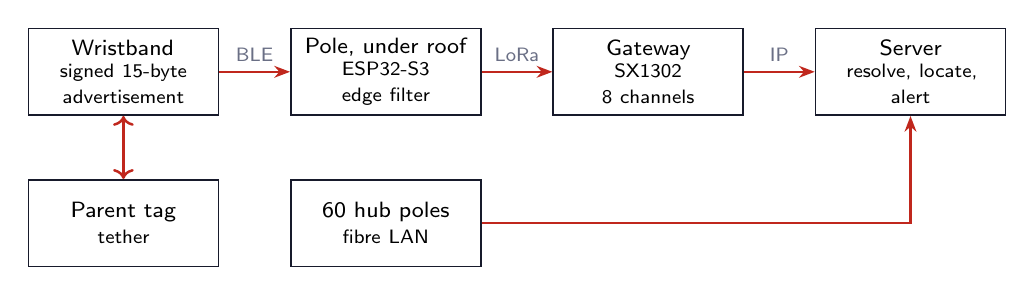
\begin{tikzpicture}[node distance=5mm,every node/.style={font=\sffamily\footnotesize,align=center},
 box/.style={draw=rsink,line width=0.6pt,minimum height=11mm,text width=22mm,inner sep=3pt},
 arr/.style={-{Stealth[length=2mm]},rsred,line width=0.9pt}]
\node[box](band){Wristband\\\scriptsize signed 15-byte\\\scriptsize advertisement};
\node[box,right=9mm of band](pole){Pole, under roof\\\scriptsize ESP32-S3\\\scriptsize edge filter};
\node[box,right=9mm of pole](gw){Gateway\\\scriptsize SX1302\\\scriptsize 8 channels};
\node[box,right=9mm of gw](srv){Server\\\scriptsize resolve, locate,\\\scriptsize alert};
\draw[arr](band)--node[above,text=rsmuted,font=\sffamily\scriptsize]{BLE}(pole);
\draw[arr](pole)--node[above,text=rsmuted,font=\sffamily\scriptsize]{LoRa}(gw);
\draw[arr](gw)--node[above,text=rsmuted,font=\sffamily\scriptsize]{IP}(srv);
\node[box,below=8mm of pole](fib){60 hub poles\\\scriptsize fibre LAN};
\draw[arr](fib.east)-|(srv.south);
\node[box,below=8mm of band](tag){Parent tag\\\scriptsize tether};
\draw[arr,<->](band)--(tag);
\end{tikzpicture}
\caption{The data path. A pole listens below the roof and transmits above it. The 60 poles of the two crowded hubs
bypass radio and use the shrine's fibre network.}\label{fig:path}\end{figure}

\textbf{The wristband} is a coin-cell Bluetooth beacon in a sealed strap, issued at registration to a child or an
elder and returned at the exit. It has a button for SOS, a buzzer and a light. It does not know where it is. It sends
the same short message every 800~ms: who I am in this quarter of an hour, how my battery is, whether my button is
pressed, and a signature.

\textbf{The parent tag} is the same hardware with a different role. It carries a list of the child band's next
identifiers and buzzes when it stops hearing them.

\textbf{The pole} is a small box clamped under the shelter roof on an existing light pole: an ESP32-S3 that scans for
wristbands, and an SX1262 LoRa radio whose antenna is led through the roof. It keeps a table of the wristbands in
range and decides what is worth sending. It holds no secret that identifies anyone.

\textbf{The gateways}, six of them on hilltops, receive the poles' uplinks on eight channels and pass them to an
on-premise server. \textbf{The server} holds the keys, the pairing records and the map of the route. It turns an
anonymous identifier heard at pole~175 into ``the child registered with family 0421 is on the Sanjichhat track, 243~m
from her parent'', and raises alarms.

\section{The route in the model}
\begin{table}[htb]\centering\small\caption{Zones of the model route. Lengths and the pole total are the white paper's;
positions within a zone are schematic.}\label{tab:zones}\TableZones\end{table}
\begin{figure}[htb]\centering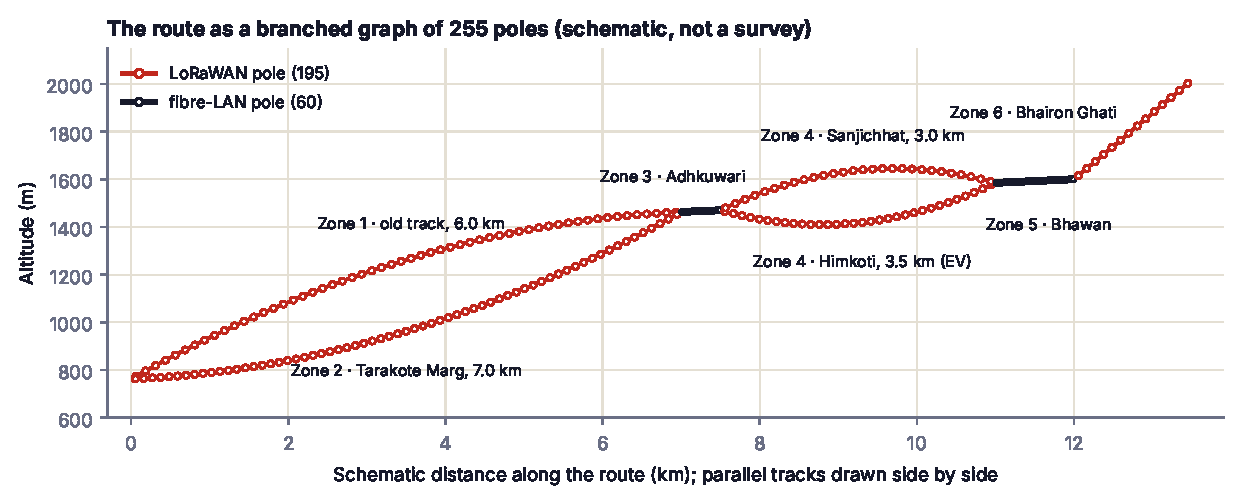
\includegraphics[width=\linewidth]{trek}
\caption{The model route. Zone~4 is two parallel tracks; their split of 6.5~km into 3.5 and 3.0~km is assumed.}\label{fig:trek}\end{figure}
The 195 LoRaWAN poles cover 21.0~km, one per 108~m on average. The first draft said poles stand ``every 25 to 100~m'';
with 255 poles in all, 25~m in the hubs and about 108~m on the tracks is what fits. Chapter~\ref{ch:radio} shows that
the radio range allows it.

\FloatBarrier
% ====================================================================================================
\chapter{The signed advertisement}\label{ch:frame}
\hook{Fifteen bytes that say who is here to the server, and nothing to anyone else.}
\section{Who might attack a child's wristband}
A system that tracks children must be designed against people who would misuse it. Four are considered.
\begin{itemize}
\item $\mathcal A_1$, the \textbf{stalker}, places cheap receivers along the path and tries to follow one wristband, or
to learn which wristbands travel together.
\item $\mathcal A_2$, the \textbf{replayer}, records advertisements and broadcasts them again somewhere else or later,
to create false sightings or false alarms.
\item $\mathcal A_3$, the \textbf{forger}, sends commands to a wristband to make it buzz or to flatten its battery.
\item $\mathcal A_4$, the \textbf{thief}, takes a pole or a wristband apart to read keys from its memory.
\end{itemize}

\section{Keys}
The server keeps one 128-bit master key, $\Kmaster$, in an encrypted keystore or a hardware security module. Each
wearable gets its own key when it is made,
\begin{equation}K_u=\cmac{\Kmaster}{\mathrm{UID}_u\,\|\,\mathrm{Salt}},\end{equation}
and its debug port is locked. If $\mathcal A_4$ extracts $K_u$ from one wristband, that wristband is compromised and
no other. A pole never receives $\Kmaster$ or any $K_u$, so a stolen pole reveals no identities. The pole has its own
LoRaWAN keys, and those are worth protecting too, with secure boot and encrypted flash, because they let it speak to
the network.

\section{A counter instead of a clock}
The wearable has no clock set to the time of day, and setting one would mean a two-way Bluetooth connection at the
registration desk, which is slow in a queue. It keeps a 16-bit counter $c$ instead, stepped every 900~s by its
32.768~kHz crystal, and \emph{sends the counter in every frame}. The registration pad only has to listen once.

\section{The frame}
In slot $c$ the wearable computes an identifier and a radio address,
\begin{align}\mathrm{ID}_{u,c}&=\operatorname{Trunc}_{32}\cmac{K_u}{\texttt{0x01}\,\|\,c},\\
M_{u,c}&=\operatorname{Trunc}_{46}\cmac{K_u}{\texttt{0x02}\,\|\,c}\ \text{with both top bits set,}\end{align}
and broadcasts the 15 bytes of Table~\ref{tab:frameb} as manufacturer data.
\begin{table}[htb]\centering\small\caption{The 15-byte payload.}\label{tab:frameb}
\begin{tabular}{@{}llp{0.60\linewidth}@{}}\toprule Bytes & Field & Content\\\midrule
0--1 & Company\_ID & \code{0xFF5A}, a laboratory value; sent low byte first\\
2 & V\_type & bits 0--3: version 4. Bit 4: 0 for a band, 1 for a parent tag\\
3--4 & Slot\_Counter & $c$, little-endian\\
5--8 & Rolling\_ID & $\mathrm{ID}_{u,c}$\\
9 & F\_stat & bit 0 SOS pressed; bit 1 tether lost; bit 2 buzzer on; bit 3 low battery\\
10 & B\_mv & supply voltage in steps of 20~mV (150 means 3.00~V)\\
11--14 & MIC & $\operatorname{Trunc}_{32}\cmac{K_u}{\text{bytes }2\ldots10}$\\\bottomrule\end{tabular}\end{table}

\subsection*{A worked example}
Take the tag key \code{00 01 02 \ldots{} 0f}, slot 17, SOS pressed, battery 3.00~V. The reference implementation gives
\begin{center}\code{5a ff\ \ 04\ \ 11 00\ \ 3c 34 fd c9\ \ 01\ \ 96\ \ 8c 83 e4 2f}\end{center}
and the radio address \code{d4:1b:8a:54:a8:dc}. The command \code{rakshasutra frame --key 000102\ldots0f --counter 17
--sos} prints this, and the C firmware core produces the same bytes: a test compares the two on 200 random keys.

\subsection*{Three encodings the first draft left open}
The paper wrote $\operatorname{Trunc}_{32}$ and ``$\texttt{0x01}\,\|\,c$'' without saying which bytes. An
implementation must choose, and two implementations must choose alike. The reference code fixes: truncation keeps the
\emph{leading} bytes of the CMAC, as RFC~4493 does; the counter enters each CMAC as the same two little-endian bytes it
has on air; and the address is the first six CMAC bytes with the two most significant bits set, which is what marks a
static random address in Bluetooth. These are listed as \textsc{defined} in the parameter table of
Appendix~\ref{app:params}.

\section{How the server knows who it is}
At registration the pad hears one frame, checks its MIC, and stores the counter it saw, $c_{init}$, and the time,
$t_{pair}$. Afterwards the server expects, at time $t$,
\begin{equation}\hat c_u(t)=\Bigl(c_{init}+\Bigl\lfloor\tfrac{t-t_{pair}}{900}\Bigr\rfloor\Bigr)\bmod65536.\end{equation}
A crystal accurate to 20 parts per million drifts 1.7~s a day, so the wearable may step its counter a little before or
after the server expects. The server therefore keeps three identifiers per wearable, for slots $\hat c_u-1$, $\hat c_u$
and $\hat c_u+1$, in a hash map from identifier to wearable. Resolving a report is one lookup.

\begin{finding}\textbf{Identifiers can clash.} The first draft treated the map as one-to-one. With 10,000 wearables and
three slots each there are 30,000 entries drawn from $2^{32}$ values, and by the birthday bound the chance that some
two coincide at a given moment is $1-\exp(-n(n-1)/2^{33})\approx\Clash\%$. The reference server keeps a list per
identifier and uses the counter in the report to tell clashing entries apart. \lbl{calculated}\end{finding}

\section{What an eavesdropper learns}
AES-CMAC is a pseudorandom function: without the key, its outputs for different inputs look like independent random
strings. So to $\mathcal A_1$ the identifier and address of one slot have no visible connection to those of the next. A
wristband can be followed for at most the remainder of one 15-minute slot, about 1.1~km of walking. Two things soften
even that. The battery byte and the counter are sent in clear, and a counter that happens to be unusual could help
link slots; a later revision should mask the counter. And all the wristbands of a family rotate at different instants,
which hides who travels with whom from a casual listener, though not from one who watches rotations closely.

\section{What a forger can and cannot do}
The MIC covers every byte that matters, so $\mathcal A_2$ and $\mathcal A_3$ cannot alter a frame: a test flips each of
the 104 bits of bytes 2 to 14 in turn and checks that verification fails every time. Guessing a 32-bit MIC succeeds
once in $2^{32}$ tries, and a pole forwards at most ten SOS frames a minute, so a brute-force attack on one pole would
need about 800 years on average.

\begin{finding}\textbf{A limit of the design: ordinary sightings are not authenticated.} To save airtime a pole reports
an arrival as 8 bytes: identifier, counter, signal strength, flags. The MIC is left behind, and the pole, holding no
key, could not have checked it anyway. So a frame recorded near one pole and replayed near another, inside its
three-slot window of up to 45 minutes, is believed. It cannot raise an alarm, because an SOS travels as the whole frame
and is verified. But it can put a child's marker in the wrong place. The reference server flags any sighting that
implies an impossible speed, which catches a careless replay and not a careful one. The remedy is to carry the 4-byte
MIC in each arrival tuple and verify it at the server; the cost in airtime is worked out in Chapter~\ref{ch:edge}.
The repository's example \code{attack\_log.csv} shows all of this: forged alarms dropped, stale frames dropped, and
one same-slot replay accepted and flagged.\end{finding}

% ====================================================================================================
\chapter{Radio under a steel roof}\label{ch:radio}
\hook{The roof that keeps the rain off also keeps the signal in. Use both sides of it.}
\section{The model}
Received power falls with distance. The standard description is a straight line on a logarithmic scale:
\begin{equation}P_{rx}(d)=P_{tx}+G_{tx}+G_{rx}-PL(d_0)-10\,n\log_{10}(d/d_0)-L_{body}-X_\sigma.\label{eq:pl}\end{equation}
$PL(d_0)$ is the loss at a reference distance $d_0=1$~m. The exponent $n$ is 2 in free space; a corridor with a
reflecting roof can guide the signal and keep $n$ near 2 even among obstacles. $L_{body}$ is what a crowd absorbs, and
$X_\sigma$ is a random term, normally distributed in decibels with standard deviation $\sigma$, for everything the
line does not capture. The white paper's values are $P_{tx}=+8$~dBm, $PL(1\,\mathrm m)=40.2$~dB, $n=2.15$,
$L_{body}=14$~dB and $\sigma=4.2$~dB. \textbf{None has been measured under a shelter.} They are plausible design
values, and everything in this chapter is conditional on them.

\section{From margin to range}
A frame is received if $P_{rx}$ exceeds the receiver's sensitivity $S$. The \emph{margin} is the median received power
minus $S$. With the random term, a frame at margin $m$ is received with probability $\Phi(m/\sigma)$, where $\Phi$ is
the normal distribution function. For 98\% delivery the margin must be $2.05\sigma=8.6$~dB. Solving
Eq.~\ref{eq:pl} for the distance at which that margin is left gives the reliable range.

For Coded PHY at $S=-103$~dBm and 50~m:
\[P_{rx}=8-40.2-21.5\log_{10}50-14=-82.7\ \mathrm{dBm},\qquad m=\MarginFifty\ \mathrm{dB}.\]
The first draft stated 28.6~dB. The difference, 8.3~dB, would need antenna gain that the paper never specifies, and a
wristband antenna is more likely to lose a few decibels than to gain eight. This book uses \MarginFifty~dB.

\begin{table}[htb]\centering\footnotesize\caption{Link budget from Eq.~\ref{eq:pl} \lbl{calculated}. Bluetooth rows: the
distance at which 98\% of frames clear the sensitivity. LoRa rows: margin at 8~km behind one assumed 20~dB ridge.}\label{tab:linkb}
\TableLink\end{table}
\begin{figure}[htb]\centering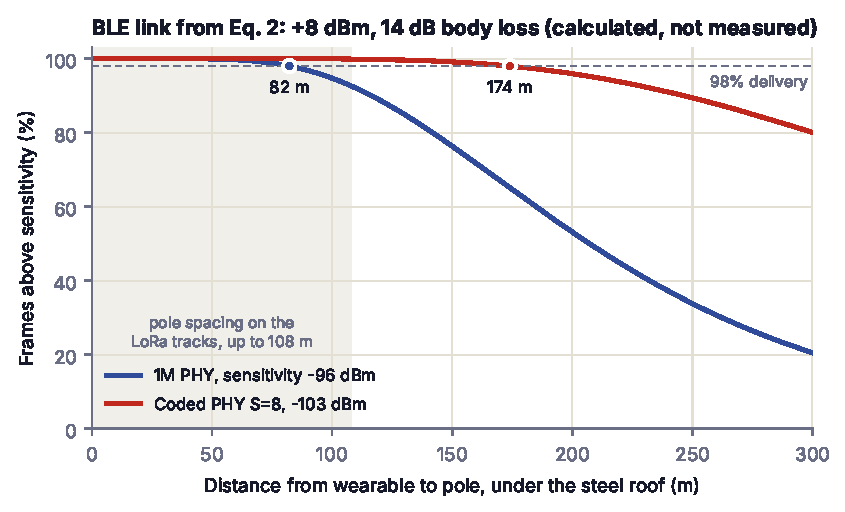
\includegraphics[width=0.78\linewidth]{link}
\caption{Share of frames above sensitivity against distance.}\end{figure}

The ranges, \RangeOneM~m on 1M PHY and \RangeCoded~m on Coded PHY, are longer than the 28.5~m and 92~m the first draft
tabled; its table does not follow from its own equation. The conclusion survives either way: Coded PHY covers poles
108~m apart, and 1M PHY would not with any comfort.

\section{Why the pole is split}
Mount the whole pole above the roof, and the Bluetooth signal from a wrist below must pass through steel: 24.1~dB lost
by the design value. With a $+4$~dBm, 1M PHY wristband the reliable range collapses to \RangeAbove~m. Mount the whole
pole below the roof, and the LoRa signal must pass through steel on its way to the hilltop: 18.4~dB lost, and the
maximum allowable path loss falls from \Mapl~dB to \MaplUnder~dB.

The split-antenna pole avoids both. The electronics and the Bluetooth antenna sit under the roof truss, looking down
at the crowd. One metre of thin coaxial cable, costing 0.9~dB, takes the LoRa signal through a sealed gland to a whip
antenna above the ridge.

The maximum allowable path loss follows directly:
\[\mathrm{MAPL}=14-0.9+5.8+126.5=\Mapl\ \mathrm{dB}.\]
How far that reaches depends on the valley, and the white paper gave ranges of 5.4 to 8.8~km without a model to derive
them from. This book claims no range. As an indication only: free-space loss at 866~MHz over 8~km is 109.3~dB; add one
ridge in the way at an assumed 20~dB, and the split antenna keeps \MarginEightOver~dB in hand at SF7, while the antenna
under the roof is \MarginEightUnder~dB short. \lbl{calculated, with an assumed ridge}

\section{The gate that defines ``here''}
A pole hears wristbands far beyond its own stretch of path. To report a wristband as \emph{here} it requires a signal
above a gate: $-75$~dBm on the tracks, $-65$~dBm in the hubs. By Eq.~\ref{eq:pl} these correspond to about
\GateTrackM~m and \GateHubM~m. That is the meaning of the ``25~m core zone'' used in Chapter~\ref{ch:move}.

\begin{finding}\textbf{What to measure first.} Three numbers carry this whole chapter: the roof loss at 2.44~GHz and at
866~MHz, and the exponent $n$ under the roof. All can be measured in an afternoon with two development boards and a
tape measure under any GI shed. Until they are, treat every range here as a hypothesis.\end{finding}

% ====================================================================================================
\chapter{Airtime}\label{ch:air}
\hook{Every report costs milliseconds on a shared channel. Count them.}
\section{How long a LoRa frame lasts}
LoRa trades speed for range. At spreading factor $SF$ and bandwidth $BW$ one symbol lasts
$T_{sym}=2^{SF}/BW$: 1.024~ms at SF7 and 125~kHz. A frame is a preamble, a header and the payload, coded so that
four bits travel as five at coding rate 4/5. For a physical payload of $PL$ bytes with an explicit header and a CRC,
the number of payload symbols is
\begin{equation}n_{pay}=8+\max\Bigl(\Bigl\lceil\frac{8\,PL-4\,SF+44}{4\,SF}\Bigr\rceil\cdot5,\;0\Bigr),\end{equation}
and the whole frame lasts $T=T_{sym}\,(n_{pre}+4.25+n_{pay})$ with a preamble of $n_{pre}=8$ symbols. LoRaWAN wraps the
application payload of $B$ bytes in 13 bytes of its own, so $PL=13+B$.

\subsection*{Worked through for an SOS}
$B=15$, so $PL=28$. The bracket is $(224-28+44)/28=8.57$, rounded up to 9; times 5 is 45; plus 8 is 53 payload
symbols. With the preamble, $8+4.25+53=65.25$ symbols, and $65.25\times1.024=\ToaSos$~ms. The same steps give
\ToaBloom~ms for 64 bytes and \ToaChunk~ms for 200 bytes. All three match the first draft exactly, and the firmware's
own calculation agrees to a microsecond. At SF9 the SOS frame takes \ToaSosNine~ms.

\section{Collisions}
Poles do not coordinate. Each transmits when it has something to send, on a channel picked at random. This is the
\emph{pure ALOHA} scheme, and its arithmetic is short. Suppose frames of length $T$ start at random at rate $\lambda$
per second on one channel. A given frame is destroyed if another starts in the $T$ seconds before it or the $T$ seconds
during it: a window of $2T$. The number of such starts is Poisson with mean $2\lambda T$, so the frame survives with
probability $e^{-2\lambda T}$. Writing $G=\lambda T$ for the offered load,
\begin{equation}P_{loss}=1-e^{-2G}.\end{equation}
With $M$ channels the load on each is the total airtime per second divided by $M$.

When frames have different lengths, a frame of length $T_i$ is destroyed by a frame of type $j$ that starts within
$T_j$ before it or $T_i$ after it starts. Summing over types,
\begin{equation}P_{loss,i}=1-\exp\Bigl(-\frac{1}{M}\Bigl(T_i\sum_j\lambda_j+\sum_j\lambda_jT_j\Bigr)\Bigr).\end{equation}
Long frames are lost more often than short ones. In a 3,000-wearable surge a 25-tag chunk is lost \LossChunk\% of
the time while the short SOS frame is lost \SosFirstLoss\% of the time.

Two real effects are left out, and both help: a strong frame can survive a weak one (capture), and different
spreading factors interfere only partly. The losses in this book are therefore pessimistic.

A note on rules. The first draft spoke of duty-cycle limits. The LoRaWAN regional parameters for IN865 set a maximum
payload and transmit power but, unlike the European band, no duty cycle. The binding limits here are the 222-byte
payload and the collisions themselves.

% ====================================================================================================
\chapter{The edge filter and the capacity of a cell}\label{ch:edge}
\hook{A pole hears a wristband a hundred times in a minute. It needs to say so once.}
\section{What a pole does}
\begin{algo}{The edge filter (Algorithm 2 of the white paper)}
\textbf{On each advertisement} with signal strength $r$:\par
1.\ Ignore it unless it is 15 bytes with Company\_ID \code{0xFF5A}.\par
2.\ If the SOS bit is set, fewer than 10 SOS frames went out this minute, and this identifier was not forwarded in the
last 90~s: send the frame now, confirmed, on port 10, with one byte of $r$ appended.\par
3.\ If $r$ is below the gate, stop.\par
4.\ Update the table entry: smoothed signal $\leftarrow0.75\cdot$old$+0.25\,r$; count the hit; note the time.\par
5.\ When the hits reach $H$ (1 on tracks, 3 in hubs) and the arrival is unreported: queue 8 bytes (identifier,
counter, signal, flags).\par
\textbf{Every 15 s}, after a random 200 to 1500~ms: retire entries unheard for 90~s; send queued arrivals in chunks of
at most 25 (200 bytes) on port 1; send departures, 4 bytes each, on port 2.\par
\textbf{Every 60 s}: send a 64-byte Bloom filter of everyone present on port 3.
\end{algo}
The table holds 1,024 entries in about 45~kB of static memory. The C implementation and the Python reference are fed
the same ten busy minutes, sixty wristbands arriving, leaving and pressing SOS, and must emit identical uplinks.

Step~2's extra byte is new. In the end-to-end simulation of Chapter~\ref{ch:server} one SOS was heard by seven poles
up to 220~m away, because Coded PHY carries far. Without a signal strength the server would pin the alarm on whichever
uplink arrived first.

\section{A model of one cell}
Take $N$ wristbands in the area served by one gateway, with $K=60$ poles, each wristband reaching a new pole every
$\tau=55$~s on average. Then:
\begin{itemize}
\item arrivals at one pole are a Poisson process of rate $N/(\tau K)$, so in a 15~s window a pole collects a Poisson
number of arrivals with mean $15N/(\tau K)$: 2.3 for $N=500$ and 13.6 for $N=3{,}000$;
\item a pole holds, on average, $N/K$ wristbands: 8 to 50.
\end{itemize}
Four designs turn this into frames.
\begin{description}
\item[Raw forwarding.] Every ping heard becomes an uplink of about 7 bytes. The first draft's table assumed a ping every
2~s.
\item[Single-event arrivals.] One 8-byte uplink per arrival, and every 60~s a list of the 4-byte identifiers present.
\item[15 s batching.] Arrivals are collected for 15~s and sent together; the same raw list every 60~s.
\item[Rakshasutra.] Arrivals in chunks of at most 25; departure lists; a 64-byte Bloom filter in place of the raw list.
\end{description}
For each, the expected airtime per second is summed over the Poisson distribution of how many items each report
carries, using the exact time on air of each frame size, and divided by 8 channels to give $G$.

\begin{table}[htb]\centering\footnotesize\caption{Offered load and frame loss, ``$G$ / loss'' in percent, for one
cell of 60 poles and 8 channels at SF7 \lbl{calculated}.}\label{tab:capb}\TableCapacity\end{table}
\begin{figure}[htb]\centering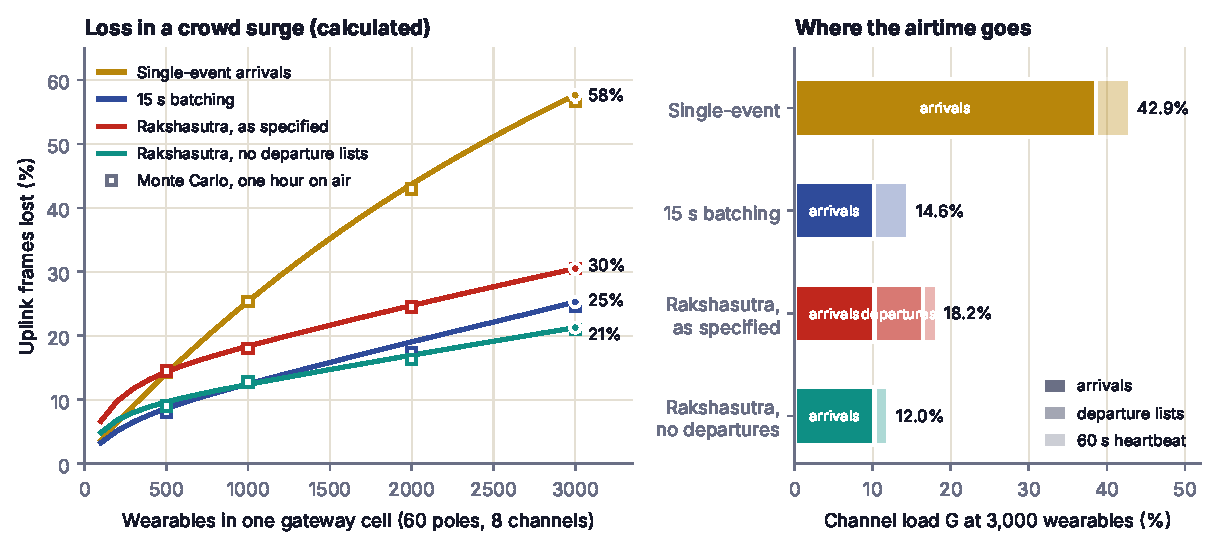
\includegraphics[width=\linewidth]{capacity}
\caption{Left: loss against the number of wristbands in the cell; squares are the Monte Carlo check. Right: the airtime
of each design at 3,000 wristbands, by stream.}\label{fig:capb}\end{figure}

\section{Checking the formula by brute force}
A formula for collisions deserves a check that does not use the formula. The simulator gives every pole its real
timers, with random phases and jitter, draws its arrivals, puts every frame on a random channel, and marks as lost any
two that overlap. Over one simulated hour per case, \McFrames{} frames in all, the simulated loss stays within
\McErr{} percentage points of the formula in every case. \lbl{simulated}

\section{What the table says}
\begin{table}[htb]\centering\footnotesize\caption{Frame loss, first draft against this model, for 500 / 1,000 / 2,000 /
3,000 wristbands.}\TableCapacityCompare\end{table}
\textbf{Batching does most of the work.} Sending arrivals together every 15~s instead of one by one cuts loss at 3,000
wristbands from \LossSingle\% to \LossBatch\%. A frame's fixed cost, preamble, header and 13 bytes of LoRaWAN, is paid
once for many arrivals.

\textbf{The Bloom filter is what keeps frames legal.} A raw list needs 4 bytes a wristband and overflows 222 bytes
beyond 55 wristbands. At $N=3{,}000$ a pole holds 50 on average, and by the Poisson distribution \OversizeBatch\% of
poles hold more than 55 at any moment. A crowd sheltering from rain would do far worse. The filter is 64 bytes always.
It also costs less airtime than raw lists once a cell holds more than about \BloomPays{} wristbands; below that, raw
lists are shorter.

\textbf{Departure lists cost more than they save.} This was the surprise of the audit. The design as specified loses
\LossRak\% of frames at 3,000 wristbands, \emph{more} than plain batching, because each pole also sends a departure
list every 15~s. Yet a departure is already implied: the wristband arrives at the next pole, and it vanishes from the
heartbeat. Dropping port~2 cuts the load from \LoadRak\% to \LoadRakNd\% and the loss to \LossRakNd\%.

\begin{finding}\textbf{The first draft's headline figure does not stand.} It gave 15.8\% loss at 3,000 wristbands and
an 82.4\% cut in airtime. Counting all the traffic of its own algorithm gives \LossRak\%, or \LossRakNd\% without
departure lists, and an airtime cut of \AirRed\% or \AirRedNd\% against single-event forwarding. The design still wins
clearly, by a smaller margin than claimed.\end{finding}

\textbf{The deployed layout is easier than the worst case.} Sixty poles to a gateway was a stress test. With 195 LoRa
poles on six gateways a cell has about \DepPoles{} poles, and with 5,000 wristbands spread over the route it holds
\DepTags{}. The loss is then \DepLoss\%, or \DepLossNd\% without departure lists; the first draft said ``well below
6\%''.

\textbf{What a lost frame costs.} Reports are unconfirmed. A lost chunk hides up to 25 arrivals at one pole; the
wristbands are seen again at the next pole about 55~s later. The chance of missing someone at $k$ poles in a row falls
as the $k$-th power of the chunk loss: with \LossChunk\% chunk loss, about one in nine is missed twice running.

\section{The Bloom filter in detail}
A Bloom filter is a row of bits, here 512. To add an item, hash it to $k=3$ positions and set those bits. To ask
whether an item is present, check its three bits. If any is clear the item is certainly absent. If all are set it is
\emph{probably} present: other items may have set them. After $n$ items a given bit is still clear with probability
$e^{-kn/m}$, so
\begin{equation}P_{false}=\bigl(1-e^{-3n/512}\bigr)^3.\end{equation}
The three positions come from two hashes, $h_1+j\,h_2$ for $j=0,1,2$, which is as good as three independent hashes for
this purpose. The reference fixes the variants the paper left open: CRC-16/CCITT-FALSE for $h_1$ and 32-bit FNV-1a
for $h_2$.
\begin{figure}[htb]\centering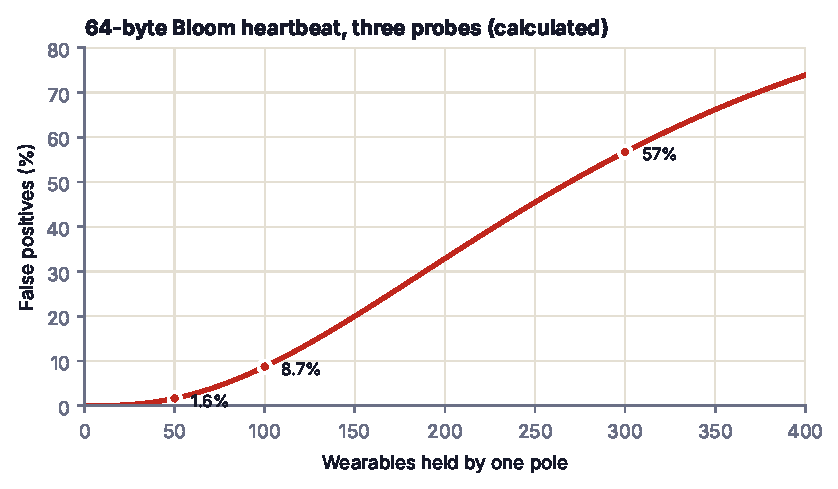
\includegraphics[width=0.74\linewidth]{bloom}\caption{False positives of the 64-byte
heartbeat \lbl{calculated}; a test confirms the curve by direct counting.}\end{figure}

The rate is \BloomFifty\% at 50 wristbands, \BloomHundred\% at 100 and \BloomThree\% at 300. Sixty-four bytes hold
about \BloomCapOne{} wristbands at 1\% and \BloomCapFive{} at 5\%. Two consequences. The server must not ask a
heartbeat ``which of my 10,000 wristbands are here?'', since hundreds would falsely match; it asks only about
wristbands it already places at that pole. And at the crowded hubs the filter saturates; those poles are on fibre,
where a filter ten times larger costs nothing.

\section{The price of signing sightings}
Chapter~\ref{ch:frame} noted that arrival tuples carry no MIC. Adding it makes a tuple 12 bytes and a full chunk 16
wristbands instead of 25. That is a design choice for the next revision, and the model in the repository can cost it
by changing one parameter.

% ====================================================================================================
\chapter{People who move}\label{ch:move}
\hook{An alert is only useful if it arrives before the person has walked out of range of it.}
\section{The Class A trap}
A LoRaWAN Class~A device listens only briefly after each of its own transmissions. To reach a wristband through a
Class~A pole the server must wait for the pole's next uplink. Add up the worst case: 15~s for the arrival batch, 90~s
to be sure the separation is real, up to 60~s for the downlink window, and 8~s for the pole to open a Bluetooth
connection to the wristband. That is 173~s. At 1.25~m/s a person walks \ClassAWalk~m in 173~s. By the time the pole
tries to connect, the person is two poles further on. The alert fails every time.

\section{Layer 1: the tether}
The first layer needs no network. At pairing, the pad copies the child band's next 96 identifiers, 24 hours' worth and
384 bytes, into the parent tag. The tag listens for them. Four misses in a row, and it sounds its own buzzer.

\subsection*{The scan window}
The first draft had the tag open a 5~ms scan window every 5~s. Consider what that window can catch. The band sends an
advertisement every 800~ms, plus a random delay of up to 10~ms that Bluetooth requires, at a phase the tag does not
know. The packet the tag must catch lasts about 1.2~ms on Coded PHY. A 5~ms window contains a whole packet only if the
packet starts in its first 3.8~ms, so the chance is
\[\frac{5-1.17}{805}=\TetherHit\%.\]
Four scans in a row then all miss with probability \TetherAlarm\%. The tag would be in alarm almost all the time with
the child holding the parent's hand; in simulation, \TetherAlarmSim\% of the time. \lbl{simulated}

A window can only be certain to catch a packet if it is as long as the advertising interval, the random delay and one
packet together: \TetherWindow~ms. A receiver drawing 4.6~mA for \TetherWindow~ms in every 5~s averages
\TetherUa~\textmu A, twenty-five times the whole budget of the child's band, and would empty the parent tag's cell in
about \ParentLife{} months.

\begin{finding}\textbf{Design fix.} The tether cannot work as first specified. Two routes are open. The simple one is
the long window above, with a rechargeable parent tag. The better one is to make the listening synchronised: Bluetooth
5 periodic advertising lets a receiver wake for a few milliseconds exactly when the next packet is due. That is the
route planned for the next revision, and it would also serve the band's own scan for wake tokens.\end{finding}

\subsection*{Where the alarm sounds}
The first draft said the tether triggers at about 25 to 30~m. But the tag stops hearing the band where the radio link
ends, and by Eq.~\ref{eq:pl} that is beyond \TetherRange~m on Coded PHY. To alarm at 30~m the tag must treat
\emph{weak} as \emph{gone}: by the same equation, a signal below about $-$\TetherGate~dBm. With 4.2~dB of shadowing
such a gate will sometimes trip early and sometimes late; requiring four weak readings in a row steadies it.

\section{Layer 2: a wake token from the poles}
The second layer covers what the tether cannot: a parent tag that has failed, a guard starting a search, a separation
discovered by the server because two wristbands of one family are at poles far apart. All poles keep their LoRa
receivers open continuously (Class~C), and the server multicasts an 8-byte token to the poles within two hops of the
wristband: five poles on a plain stretch, more at a junction. They broadcast it by Bluetooth, and the wristband buzzes.

The token is the current identifier, a command byte, and the first 24 bits of an AES-CMAC under $K_u$ over the
byte \code{0x03}, the counter and the command. The paper fixed only the sizes; this layout is the reference
code's. A wristband accepts a token only for its current slot and at most once in 30~s, so a recorded token is useless
after at most 15 minutes and cannot be used to drain a battery quickly.

The first draft promised 2.5 to 5~s from decision to buzzer. That has not been calculated here, and it should not be
believed yet, because the wristband hears the token through a 5~ms scan window every 4~s: the same timing problem as
the tether, to be solved the same way.

\section{Passengers at 20 km/h}
Electric vehicles carry pilgrims along the Himkoti track at a steady 20~km/h, 5.56~m/s. A passenger crosses a pole's
25~m core zone in 4.5~s.

Many beacons save power with an accelerometer: still, they advertise slowly. But a passenger in a vehicle moving at
constant speed feels no acceleration, and the band stays in its slow mode, one advertisement every 2 to 5~s. In 4.5~s
it sends two frames, perhaps three. A hub-style rule of three hits then reports at most \SlowTwo\% of passes.

Rakshasutra removes the accelerometer, fixes the interval at 800~ms, and lets poles on transit tracks report after a
single decoded frame. A pass then holds five or six frames and needs one. Whether a frame is decoded depends on the
crowd: a pole's scanner hears all wristbands in range on the same channel, and two packets that overlap are both lost.
With $n$ others in range, each sending a 1.2~ms packet every 800~ms, a frame survives with probability
$e^{-2n\times1.17/800}$.
\begin{figure}[htb]\centering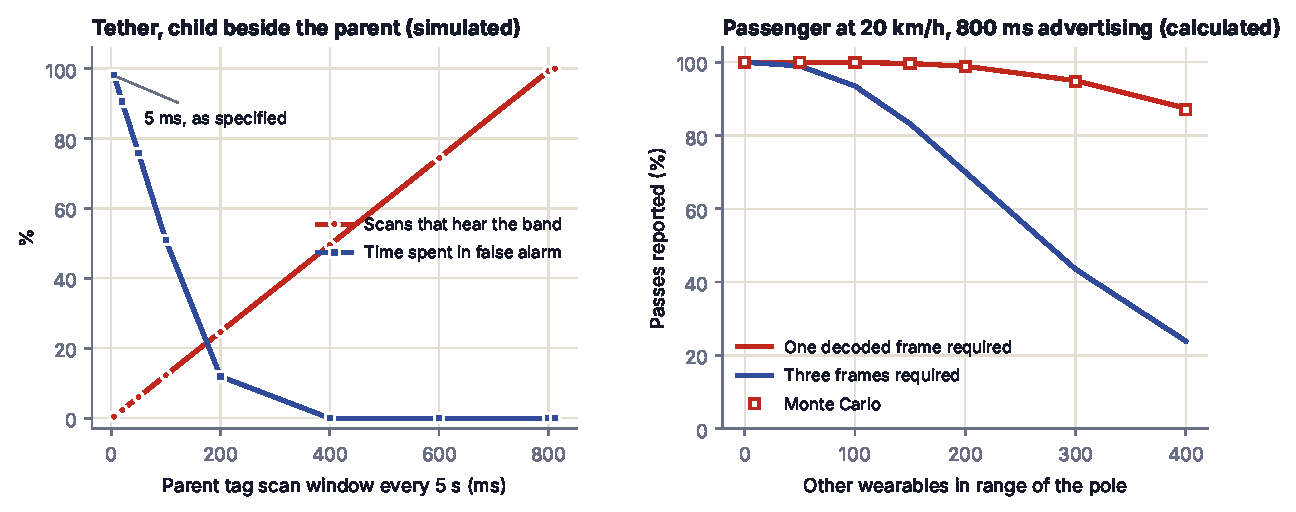
\includegraphics[width=\linewidth]{tether_ev}
\caption{Left: the tether, with the child beside the parent \lbl{simulated}. The dip to zero false alarms between 400
and 800~ms is a beat between the 5~s and 800~ms periods and should not be relied on. Right: capture of a passenger
\lbl{calculated, with a Monte Carlo check}.}\end{figure}
The capture rate is \EvCap\% with 150 other wristbands in range of the pole, the figure closest to the first draft's
99.4\%, and \EvCapDense\% with 300. It is not a single number: it falls as the crowd grows. This simple collision
model also ignores how an ESP32 scanner follows extended advertisements onto secondary channels, which will cost
something more. Scanner capacity in a dense crowd is the second thing to measure.

\section{An SOS, timed}
From button to alarm: wait for the next advertisement, at most 200~ms once SOS is pressed; decode at a pole; one LoRa
frame of \ToaSos~ms; and the backhaul. If the uplink collides, the pole repeats it at SF9 after its acknowledgement
window. The wait before a repeat, about 3~s, is assumed here.

In simulation under the 3,000-wristband surge, the first attempt is lost \SosFirstLoss\% of the time. The median delay
is \SosMedian~s; \SosFour\% of alarms arrive within 4~s; 95\% within \SosPninefive~s. With 500 wristbands in the cell
\SosFourLow\% arrive within 4~s. On the fibre poles of the hubs, 95\% arrive within \SosFiberP~s. \lbl{simulated}

The first draft promised ``sub-4-second'' latency in its abstract and ``sub-5-second'' in its conclusion. What the
model supports is: usually half a second, and within four seconds about nine times in ten under the worst surge.
Giving SOS its own channel, kept clear of routine traffic, would close most of the gap and is worth one of the eight.

% ====================================================================================================
\chapter{Power}\label{ch:power}
\hook{A coin cell, a year of pilgrimages, and one cold night with the buzzer on.}
\section{The budget}
A wristband spends nearly all its time asleep, waking briefly to transmit. Its mean current is the sum, over each
activity, of peak current times the fraction of time spent in it.
\begin{table}[htb]\centering\footnotesize\caption{Current budget of the wristband, from the first draft's Table~V
(design values, to be re-derived for the chosen chip).}\TablePower\end{table}
The total, \Iactive~\textmu A, reproduces the first draft. A CR2450 cell holds 620~mAh. A band spends 14 hours a day on
the trek and 10 on the storage rack, where a magnet holds a reed switch open and it draws 0.6~\textmu A. Daily
consumption is $14\times\Iactive+10\times0.6=422$~\textmu Ah, so the cell lasts
\[\frac{620{,}000}{422}=1{,}468\ \text{days}=\LifeWarm\ \text{months}.\]
In the cold a lithium cell gives up less of its charge; with the paper's 30\% derating at $-5$~\textdegree C the life
is \LifeCold{} months. The first draft stated 14.2 and 11.1 months, which do not follow from its own table.

\section{Coded PHY costs airtime}
There is a second problem with the table, and it works the other way. It allows 1.25~ms of transmission per
advertisement. Count the bits. A legacy advertisement at 1~Mbit/s with a 15-byte payload is 33 bytes on air, 0.264~ms,
sent on three channels: \AdvOneM~ms. That fits 1.25~ms with room for the radio to start up.

But the range in Chapter~\ref{ch:radio} assumed Coded PHY, which sends every bit eight times. Coded advertising also
uses the extended format: a short pointer packet on each of the three primary channels, then the data on a secondary
channel. Each packet has a 0.376~ms preamble and access code and then 64~\textmu s per byte:
\begin{center}\small\begin{tabular}{@{}lrr@{}}\toprule Packet & PDU bytes & On air (ms)\\\midrule
\code{ADV\_EXT\_IND}, three times & 9 & $3\times1.168$\\
\code{AUX\_ADV\_IND}, once & 29 & 2.448\\\midrule Total && \AdvCoded\\\bottomrule\end{tabular}\end{center}
At \AdvCoded~ms per event the advertising current rises from 22 to 106~\textmu A, the total to
\IactiveCoded~\textmu A, and the battery life falls to \LifeWarmCoded{} months at 25~\textdegree C and
\LifeColdCoded{} months at $-5$~\textdegree C. \lbl{calculated}
\begin{figure}[htb]\centering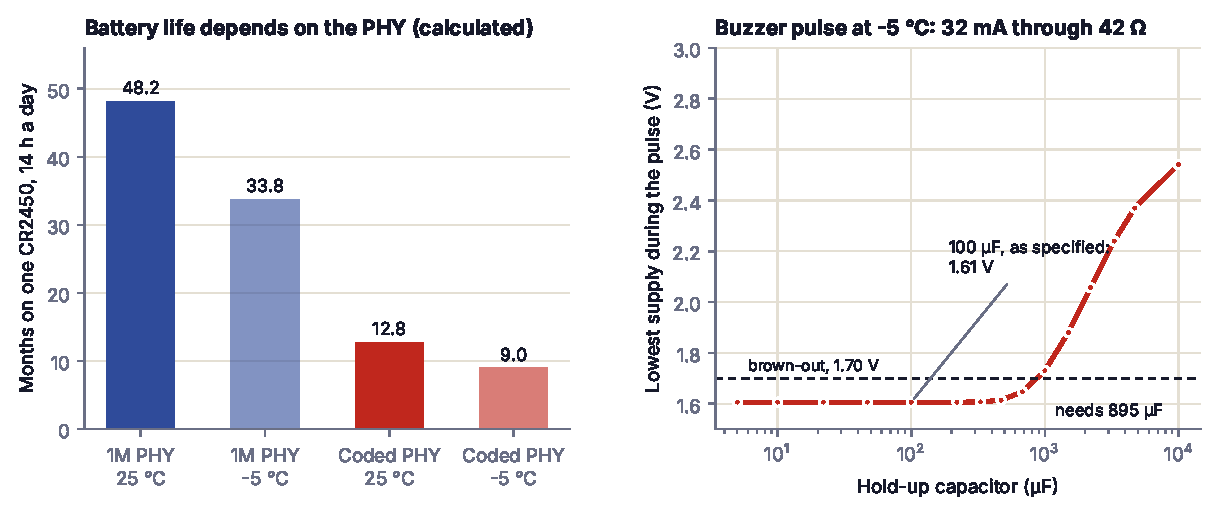
\includegraphics[width=\linewidth]{power}
\caption{Left: battery life. Right: the supply during a buzzer pulse in the cold, against the hold-up capacitor.}\end{figure}

By coincidence the Coded PHY figure lands near the first draft's claim. The honest statement is: about a year warm
and nine months cold, with range; or about four years warm, without it. A band could use 1M PHY in the dense hubs,
where poles are 25~m apart, and Coded PHY on the long tracks.

\section{The buzzer in the cold}
At $-5$~\textdegree C the cell's internal resistance rises to about 42~$\Omega$. The buzzer and a bright LED together
draw 32~mA. Ohm's law gives the drop inside the cell: $0.032\times42=1.34$~V. A cold cell at 2.95~V then delivers
\DroopUnbuf~V, and the radio chip resets below 1.70~V. This much the first draft had right.

Its remedy was a 100~\textmu F capacitor across the supply and a 20\% duty cycle, 100~ms on and 400~ms off, with the
argument that the \emph{average} current is then 6.4~mA and the drop only 0.27~V. The argument fails because a
capacitor averages only over times shorter than its time constant. Model the cell as a voltage source $V_0$ behind a
resistance $R$, with the capacitor $C$ across the load. During a pulse of current $I$ the supply falls towards
$V_0-IR$ as
\begin{equation}V(t)=V_0-IR\bigl(1-e^{-t/RC}\bigr).\end{equation}
With $R=42~\Omega$ and $C=100$~\textmu F the time constant is \TauMs~ms. A 100~ms pulse is 24 time constants long.
The capacitor is exhausted in the first few milliseconds and the supply sits at \DroopCap~V for the rest of the pulse:
a brown-out, exactly as without it. A test in the repository integrates the circuit step by step and agrees with the
closed form.

For the supply to stay above 1.70~V through a 100~ms pulse the time constant must be about 38~ms, which needs at least
\CapNeed~\textmu F, a large part for a wristband. The simpler fix is to draw less: any pulse below \PulseMax~mA is
safe with no capacitor at all. A piezo buzzer and a more modest LED fit under that.

\section{Which chip}
The first draft specified the nRF52811 transmitting at $+8$~dBm. That chip's specified maximum is $+4$~dBm. Parts in
the same family that reach $+8$~dBm, such as the nRF52820 and nRF52833, draw about the 14~mA the table assumes. This
must be confirmed against the datasheets, and it matters twice: 4~dB less power shortens the Coded PHY range from
\RangeCoded~m to about 113~m, and a different chip changes every current in the table. It is listed as open in the
audit.

% ====================================================================================================
\chapter{The route as a graph, and the control room}\label{ch:server}
\hook{Pole 173 and pole 174 are neighbours on paper and three kilometres apart on foot.}
\section{Distance on a branching path}
Number the poles along the path and it is tempting to measure separation by subtracting pole numbers. On a path that
forks, that is wrong. The route is a graph: poles are vertices, adjacent poles are joined by edges weighted with their
distance in metres, and the separation of two people is the shortest path between their poles,
\begin{equation}d_G(p_a,p_b)=\min_{\pi}\sum_{e\in\pi}w(e),\end{equation}
found by Dijkstra's algorithm. In the model the last pole of the Himkoti track is number 173 and the first pole of the
Sanjichhat track is 174. They are \BranchExample~km apart. The graph has 255 vertices; all distances from one pole take
a fraction of a millisecond.

\section{One family, end to end}
The repository contains a simulation that exercises every part at once. A parent with a tag and a child with a band
walk the last stretch of the old track and through the Adhkuwari hub at 1.25~m/s. At the junction the parent takes the
Himkoti track and the child the Sanjichhat track. The child presses SOS 150~s later. Every advertisement is a real
signed frame. Forty-eight poles run the real edge filter. Uplinks from LoRa poles are dropped at random 12\% of the
time. The server receives \WalkUplinks{} uplinks and knows nothing else.
\begin{figure}[htb]\centering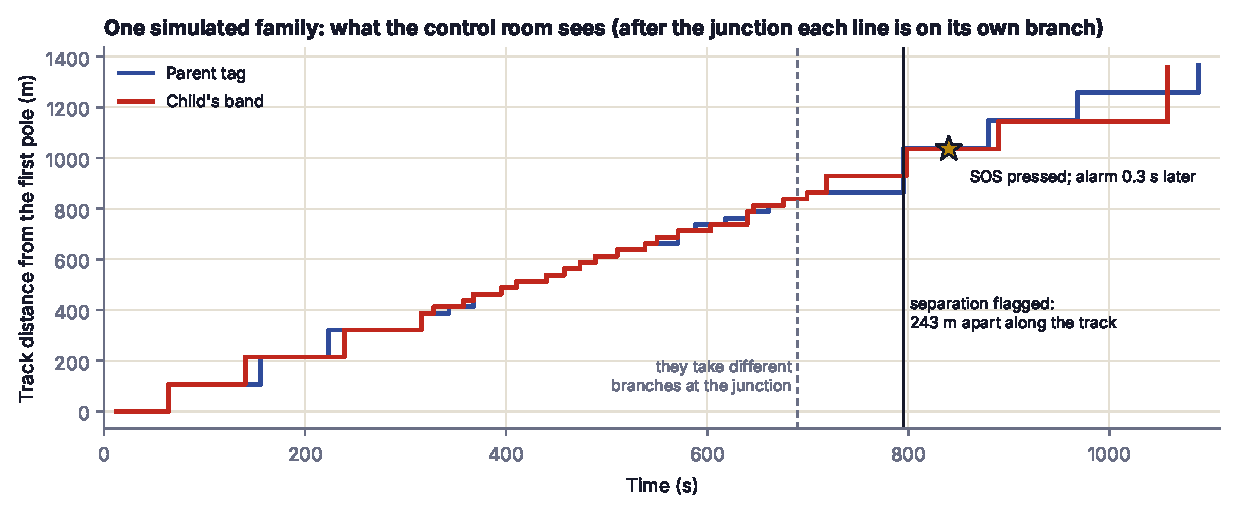
\includegraphics[width=\linewidth]{walk}
\caption{What the control room reconstructs \lbl{simulated}.}\end{figure}
The control room flags the separation \WalkSepDelay~s after the two part, when the server places them \WalkSepM~m
apart along the track, and issues wake tokens for both. When the child presses SOS, seven poles hear it; the alarm is
raised \WalkSosDelay~s later and placed, by signal strength, at the right pole. The same log is shipped as
\code{examples/adhkuwari\_separation.csv}, and
\begin{center}\footnotesize\code{rakshasutra trace examples/adhkuwari\_separation.csv \textbackslash}\\\code{\ \ \ \ --registry examples/registry.json}\end{center}
replays it.

The \WalkSepDelay~s deserve a comment. The server only alerts at 200~m of separation, and its picture of where
people are is as coarse as the pole spacing, 108~m on the tracks. Two people must be two poles apart before the
alert can fire. This is what Layer~1 is for: the tether would have noticed within 20~s.

\section{The backend}
The white paper specifies an MQTT broker to absorb bursts, in-memory resolution, and batched writes to a time-series
database. None of that is built. The reference server is a few hundred lines of Python with a dictionary where the
deployed system would have Redis. It exists to pin down behaviour, not performance.

% ====================================================================================================
\chapter{Privacy, law and physical safety}\label{ch:law}
\hook{A system that follows children has to be harder on itself than the law requires.}
\textbf{Consent and minimisation.} India's Digital Personal Data Protection Act, 2023 requires, in Section~9,
verifiable consent from a parent or guardian before a child's personal data are processed, and prohibits tracking or
behavioural monitoring of children and advertising targeted at them. Rakshasutra's purpose is the narrow one of
safety during a visit. Consent is recorded at registration. The server stores a first name, the band's identifier, a
guardian's phone number and the card number. No personal data are broadcast: an advertisement contains a pseudonym, a
counter, flags and a battery level. Location trails are deleted within 24 to 72 hours of the band's return. Whether
this use falls within an exemption or needs explicit handling under the Act's rules is a legal question to settle
with counsel before any pilot; this book does not settle it.

\textbf{Who can look someone up.} Kiosks in the phone-free zones answer only to the family's own card or parent tag,
and show only the members bound to it. There is no search by name. A kiosk locks after three failed scans, logs every
query, and blanks after 30~s. Control-room staff see more, and their queries must be logged too.

\textbf{What the design does not protect against.} Chapter~\ref{ch:frame} listed the limits: tracking within one
15-minute slot, and replay of unsigned sightings. A third is the server itself. Whoever holds the master key and the
pairing table can follow every wristband. The design assumes an on-premise server under the shrine authority's
control, with the key in hardware.

\textbf{Button cells.} A coin cell swallowed by a small child can cause severe internal burns within hours. IEC
60086-4 covers the safety of lithium cells. The band is ultrasonically welded or closed with captive tool-only screws,
has no battery door, and is retired, not opened, when its cell is spent. The strap is non-porous and is disinfected
between uses.

\textbf{Radio rules.} The 865--867~MHz band is licence-exempt in India for low-power devices within the limits set by
the Wireless Planning and Coordination Wing. Any deployment needs type-approved radios within those limits.

% ====================================================================================================
\chapter{The audit}\label{ch:audit}
\hook{Every checkable number in the first draft, recomputed.}
The first draft of White Paper WP-01 was written in October 2026. Its title called the system Rakshasutra and its text
called it SurakshaNet; it described its results as ``empirical'' and spoke of ``field propagation measurements''.
There were none. For the revised paper and this book, each number that can be checked by calculation was recomputed
by the code in the repository, using the paper's own equations and parameters.

\begin{center}\renewcommand{\arraystretch}{1.3}\begin{tabular}{@{}lrp{0.62\linewidth}@{}}\toprule
Verdict & Count & Meaning\\\midrule
reproduced & \AuditRep & the model gives the first draft's number\\
differs & \AuditDiff & the model gives another number; the revision uses the model's\\
design fix & \AuditFix & the mechanism does not work as specified; the fix is stated\\
open & \AuditOpen & needs a datasheet check or a measurement\\\bottomrule\end{tabular}\end{center}

{\footnotesize\TableAudit}

\noindent The notes on each entry are in \code{AUDIT.md} in the repository, which is generated from the same results
file as this table. The command \code{rakshasutra audit} prints it.

\section*{How this happened}
The pattern of errors is instructive. The numbers that reproduce are the ones with a formula written beside them: time
on air, the path-loss budget, the current sum, the kinematics. The numbers that fail are results stated without a
derivation: the capacity table, the ranges, the battery life. And the mechanisms that fail are the ones where an
average was trusted in place of a time scale: an average current through a capacitor too small to average it, and a
scan window compared with nothing at all. The remedy adopted here is mechanical. No number in this book, the white
paper, the README or the website is typed by hand; each is written by script from a results file, and a test fails if
a saved result no longer matches the code.

% ====================================================================================================
\chapter{Limits and next steps}\label{ch:next}
\hook{What this work is not, and what would make it more.}
\section{Limits}
\begin{itemize}
\item \textbf{Nothing is measured.} Roof loss, the path-loss exponent, body loss, shadowing, the currents: all are
design values. Every range and every lifetime depends on them.
\item \textbf{The route is schematic.} Zone lengths are the white paper's. Pole positions, altitudes within a zone and
the split of zone~4 are assumed. It is not a survey.
\item \textbf{The capacity model is simple.} Poisson movement, pure ALOHA, no capture, one spreading factor. It is
pessimistic about collisions and silent about gateway limits and downlink traffic.
\item \textbf{Bluetooth capacity is barely modelled.} One collision formula on one primary channel. A real scanner
following extended advertisements in a crowd of hundreds will do worse.
\item \textbf{Layer~2 latency is not modelled}, and the wearable's scan for wake tokens has the tether's problem.
\item \textbf{The pole sketch has not run on hardware}, and there is no wearable firmware. The C core is tested on a
host computer only.
\item \textbf{The cost figure} of INR~225--235 per band is an estimate from the first draft, not a quotation.
\item This is research software and a design study. It is not a safety system and must not be relied on as one.
\end{itemize}

\section{Next steps}
\begin{center}\small\renewcommand{\arraystretch}{1.3}\begin{tabular}{@{}p{0.25\linewidth}p{0.52\linewidth}l@{}}\toprule
Stop & Output & Status\\\midrule
Reference model & Package, firmware core, simulations, this book, WP-01 revision 2, the audit & Done\\
Protocol revision & Periodic-advertising tether; signed arrival tuples; no departure lists; SOS channel; masked counter & Next\\
Bench radio & Roof loss and range under a GI shed; scanner capacity with many beacons; currents of the chosen chip & Planned\\
Prototype & Ten bands, three poles, one gateway; the pole sketch brought up & Planned\\
Pilot & One zone, with the shrine authority's permission and a legal review & After that\\
Peer review & A paper built on measurements & After that\\\bottomrule\end{tabular}\end{center}

Three rules are fixed in advance. Measured results will be reported beside the calculated ones in this book, whichever
way they fall. Calculated and simulated results stay labelled as such. And every number in a report is written from
result files by script.

\section{An invitation}
The first measurement needs two Bluetooth development boards, a LoRa pair, and a steel shed. If you have a GI shelter
and an afternoon, or experience with dense Bluetooth scanning, or you work on crowd safety at a shrine, the
repository's issue tracker has a form for offering data or field access.

\appendix
\chapter{Parameters}\label{app:params}
Every number the models use, with its status. \textsc{paper}: a design value from the white paper, not measured.
\textsc{standard}: fixed by a specification. \textsc{defined}: an encoding this work had to fix. \textsc{assumed}: no
source; chosen so that a calculation can run. There are \Nparams{} parameters, of which \Nassumed{} are assumed and
\Ndefined{} defined here. The same table is \code{data/params.csv}.

{\scriptsize\TableParams}

\chapter{Reproducing everything}
{\footnotesize\begin{verbatim}
git clone https://github.com/0xr4j/rakshasutra.git
cd rakshasutra
pip install -r requirements.txt && pip install --no-deps -e .
make test        # the automated tests; compiles the firmware core too
make results     # every study; a few seconds, all seeds fixed
make generated   # numbers, tables, figures, AUDIT.md
make book whitepaper site
\end{verbatim}}
\begin{center}\small\begin{tabular}{@{}lp{0.62\linewidth}@{}}\toprule Path & Content\\\midrule
\code{src/rakshasutra/} & the reference model: protocol, radio, capacity, power, route, server, simulations\\
\code{firmware/} & the C core, a host test, and the pole sketch\\
\code{experiments/} & one script per study\\
\code{tests/} & the automated tests\\
\code{data/} & parameters, zones and poles\\
\code{results/} & saved output of every study\\
\code{generated/} & numbers, tables and figures written from the results\\
\code{examples/} & a family walk and an attack log to replay\\
\code{book/}, \code{whitepaper/} & the sources of this book and of WP-01\\
\code{demo/}, \code{docs/} & the browser explorer and the website\\\bottomrule\end{tabular}\end{center}

\chapter{What the tests pin down}
\begin{itemize}
\item \textbf{Cryptography.} AES-128 against the FIPS~197 vector; AES-CMAC against the four RFC~4493 vectors and
against an independent library; the frame layout byte by byte; rejection of every single-bit change.
\item \textbf{Radio and airtime.} The three time-on-air values of the paper; the ALOHA formulas; the capacity table's
headline numbers; agreement of the formula with Monte Carlo.
\item \textbf{The edge filter.} Report-once, chunking at 25, the three-hit rule, departure after 90~s, the SOS rate
limit, a bounded table.
\item \textbf{The server.} The expected counter, the three-slot window, stale and unknown identifiers, forged SOS,
signal-strength arbitration, identifier clashes, unpairing.
\item \textbf{Models.} Link budget, battery life, the RC droop against a time-stepped circuit, kinematics, the route
graph.
\item \textbf{Firmware.} The C core against the Python reference: CMAC, 200 random frames with addresses and wake
tokens, verification, time on air, and ten busy minutes of the edge filter under three configurations.
\item \textbf{The browser explorer.} Its JavaScript kernel against the Python reference.
\item \textbf{Bookkeeping.} The parameter file matches the package; the shipped examples are what the generator
writes; the saved results and the audit match a fresh calculation.
\end{itemize}

\chapter*{References}
\addcontentsline{toc}{chapter}{References}
\begin{enumerate}[leftmargin=2em,label={[\arabic*]},itemsep=3pt]\small
\item LoRa Alliance. \emph{RP002-1.0.4 LoRaWAN Regional Parameters}. 2022.
\item Semtech. \emph{LoRa Modem Designer's Guide}, AN1200.13.
\item J.~Song, R.~Poovendran, J.~Lee, T.~Iwata. The AES-CMAC algorithm. RFC~4493, IETF, 2006.
\item National Institute of Standards and Technology. \emph{Advanced Encryption Standard}, FIPS~197.
\item Bluetooth SIG. \emph{Bluetooth Core Specification}, version 5.1, 2019.
\item B.~H.~Bloom. Space/time trade-offs in hash coding with allowable errors. \emph{Communications of the ACM}
13(7):422--426, 1970.
\item A.~Kirsch, M.~Mitzenmacher. Less hashing, same performance: building a better Bloom filter. \emph{Random
Structures and Algorithms} 33(2):187--218, 2008.
\item N.~Abramson. The ALOHA system: another alternative for computer communications. \emph{Proc.\ AFIPS Fall Joint
Computer Conference}, 1970.
\item Government of India. \emph{The Digital Personal Data Protection Act, 2023} (No.~22 of 2023).
\item Wireless Planning and Coordination Wing, Government of India. Rules for low-power equipment in the 865--867~MHz
band.
\item A.~Augustin, J.~Yi, T.~Clausen, W.~M.~Townsley. A study of LoRa: long range and low power networks for the
Internet of Things. \emph{Sensors} 16(9):1466, 2016.
\item M.~Centenaro, L.~Vangelista, A.~Zanella, M.~Zorzi. Long-range communications in unlicensed bands: the rising
stars in the IoT and smart city scenarios. \emph{IEEE Wireless Communications} 23(5):60--67, 2016.
\item F.~Adelantado, X.~Vilajosana, P.~Tuset-Peiro, B.~Martinez, J.~Melia-Segui, T.~Watteyne. Understanding the
limits of LoRaWAN. \emph{IEEE Communications Magazine} 55(9):34--40, 2017.
\item A.~Heinrich, M.~Stute, T.~Kornhuber, M.~Hollick. Who can find my devices? Security and privacy of Apple's
crowd-sourced Bluetooth location tracking system. \emph{Proceedings on Privacy Enhancing Technologies} 2021(3):227--245.
\item E.~W.~Dijkstra. A note on two problems in connexion with graphs. \emph{Numerische Mathematik} 1:269--271, 1959.
\item Nordic Semiconductor. \emph{nRF52811 Product Specification}.
\item IEC 60086-4. \emph{Primary batteries, Part 4: Safety of lithium batteries}.
\end{enumerate}
\end{document}
